
\documentclass[10pt,a4paper]{article}
\usepackage{f1000_styles}

%% Default: numerical citations
% \usepackage[numbers]{natbib}

%% Uncomment this lines for superscript citations instead
% \usepackage[super]{natbib}

%% Uncomment these lines for author-year citations instead
% \usepackage[round]{natbib}
% \let\cite\citep

%% lines required to use a CSL style for references
\newlength{\cslhangindent}
\setlength{\cslhangindent}{1.5em}
\newlength{\csllabelwidth}
\setlength{\csllabelwidth}{3em}
\newlength{\cslentryspacingunit} % times entry-spacing
\setlength{\cslentryspacingunit}{\parskip}
\newenvironment{CSLReferences}[2] % #1 hanging-ident, #2 entry spacing
 {% don't indent paragraphs
  \setlength{\parindent}{0pt}
  % turn on hanging indent if param 1 is 1
  \ifodd #1
  \let\oldpar\par
  \def\par{\hangindent=\cslhangindent\oldpar}
  \fi
  % set entry spacing
  \setlength{\parskip}{#2\cslentryspacingunit}
 }%
 {}
\usepackage{calc}
\newcommand{\CSLBlock}[1]{#1\hfill\break}
\newcommand{\CSLLeftMargin}[1]{\parbox[t]{\csllabelwidth}{#1}}
\newcommand{\CSLRightInline}[1]{\parbox[t]{\linewidth - \csllabelwidth}{#1}\break}
\newcommand{\CSLIndent}[1]{\hspace{\cslhangindent}#1}

%% lines to get the code chunks working

%% lines to enable bulletpoints in a new notation style
\providecommand{\tightlist}{%
  \setlength{\itemsep}{0pt}\setlength{\parskip}{0pt}}

\begin{document}
\pagestyle{fancy}

\title{Applying a Multiverse to Habitat Analyses}
\author[1]{Benjamin Michael Marshall*}
\author[1]{Alexander Bradley Duthie**}
\affil[1]{Biological and Environmental Sciences, Faculty of Natural Sciences, University of Stirling, Stirling, FK9 4LA, Scotland, UK}

\affil[*]{\href{mailto:benjaminmichaelmarshall@gmail.com}{\nolinkurl{benjaminmichaelmarshall@gmail.com}}}
\affil[**]{\href{mailto:alexander.duthie@stir.ac.uk}{\nolinkurl{alexander.duthie@stir.ac.uk}}}

\maketitle
\thispagestyle{fancy}

\begin{abstract}

Researchers are intrinsically part of the research process. While we may strive for objectivity, there are always judgement calls required during research. When you ask 10 researchers to answer the same question with the same dataset, you will receive 10 different answers. This variation in answers has been linked to several disciplines' replication crises. Here, we explore whether answers from movement ecology, specifically habitat preference, studies vary as a result of differing analytical choices. We conducted a multiverse analysis to explore over 15,000 ways of determining habitat preference from animal tracking data. By using simulated virtual animals with a known preference, we were able to show which decisions during analysis could lead to more variable estimates of habitat preference. The multiverse revealed that data quantity (i.e., tracking frequency and duration) was more important to obtaining reliable answers than any analysis choice. Overall, the pattern of estimates shows the majority of analysis pathways provide similar final results, particularly for modern analysis methods. The pattern reflects findings from other disciplines, indicating that while movement ecology is not immune to issues of non-replicability stemming from researcher choice, it is also not at any greater risk than other disciplines.

\end{abstract}

\section*{Keywords}

Movement ecology, simulation

\clearpage
\pagestyle{fancy}

\hypertarget{introduction}{%
\section{Introduction}\label{introduction}}

Researchers are intrinsically part of the research process (\protect\hyperlink{ref-levins_dialectical_1985}{Levins \& Lewontin, 1985}; \protect\hyperlink{ref-tang-martinez_history_2020}{Tang-Martínez, 2020}), and our expectations can shape the answers we find (\protect\hyperlink{ref-holman_evidence_2015}{Holman et al., 2015}).
While we can strive to conduct research objectively, there are frequent moments during research that require judgement calls (\protect\hyperlink{ref-steegen_increasing_2016}{Steegen et al., 2016}).
Such calls, choices, or decisions occur throughout the research process, encompassing everything from study design (e.g., sample size, sampling intensity, sample stratification) to analysis (e.g., Bayesian or frequentist, ex/inclusion of outliers).
We draw on our own experience and the input of peers to try and ensure the best choices are made to produce robust and reliable results, but we also contend with data, expertise, and interpretability constraints (\protect\hyperlink{ref-liu_paths_2020}{Liu, Althoff \& Heer, 2020}).

Researchers are also influenced by the incentive system around them (\protect\hyperlink{ref-anderson_perverse_2007}{Anderson et al., 2007}).
We cannot undertake research in a vacuum; we often require institutions, funders, and scientific journals to produce and share research.
These bodies can influence what research is conducted; they are in a position to incentivise or disincentivise research of certain topics or methodologies (\protect\hyperlink{ref-fanelli_pressures_2010}{Fanelli, 2010a}; \protect\hyperlink{ref-ware_significance_2015}{Ware \& Munafò, 2015}; \protect\hyperlink{ref-smaldino_natural_2016}{Smaldino \& McElreath, 2016}).
The use of impact factor (and other similar metrics) is an example of citations being used as a measure of quality or research worth.
But when examined closer, the impact factor appears detached from the robustness or reliability of the research (\protect\hyperlink{ref-Brembs2018}{Brembs, 2018}).
This decrease in robustness can be seen in the increases in effect sizes inflation, p-value misreporting, among a number of other measures of quality (\protect\hyperlink{ref-Brembs2018}{Brembs, 2018}).
Similarly, novelty has been promoted by journals to the detriment of replications studies (\protect\hyperlink{ref-vinkers_use_2015}{Vinkers, Tijdink \& Otte, 2015}; \protect\hyperlink{ref-forstmeier_detecting_2017}{Forstmeier, Wagenmakers \& Parker, 2017}; \protect\hyperlink{ref-brembs_reliable_2019}{Brembs, 2019}), despite widespread agreement on the importance of replications (\protect\hyperlink{ref-fraser_role_2020}{Fraser et al., 2020}).
There is a bias towards positive, statistically significant results (\protect\hyperlink{ref-jennions_publication_2002}{Jennions \& Møller, 2002}; \protect\hyperlink{ref-cassey_survey_2004}{Cassey et al., 2004}).
Due to the nature of frequentist statistical significance, a prioritisation of significant results can elevate underpowered studies and boost false positive rates (\protect\hyperlink{ref-forstmeier_cryptic_2011}{Forstmeier \& Schielzeth, 2011}; \protect\hyperlink{ref-albers_problem_2019}{Albers, 2019}).

Unfortunately, there is evidence that the system of incentives trickle down to impact the judgement calls and decisions of researchers while undertaking research and when publishing those results.
The more detrimental of these decisions have been termed questionable research practices (\protect\hyperlink{ref-fraser_questionable_2018}{Fraser et al., 2018}; \protect\hyperlink{ref-bishop_rein_2019}{Bishop, 2019}).
They chiefly come in three forms: HARKing, cherry-picking, and p-hacking.
Hypothesising After Results Known (HARKing) is where the research can present the results as a confirmatory result, despite originally there being no or contrary hypothesis.
HARKing can sometimes be further enabled and rationalised by hindsight bias, where unexpected results are perceived as more likely once they have been observed (\protect\hyperlink{ref-gelman_garden_2013}{Gelman \& Loken, 2013}; \protect\hyperlink{ref-forstmeier_detecting_2017}{Forstmeier, Wagenmakers \& Parker, 2017}).
Cherry-picking is the removal or non-reporting of data points or (co-)variables, that did not yield significant results.
P-hacking is the repeated use of statistical tests, with different settings, to achieve statistical significance.
Arguably, the existence of p-hacking is enabled by an over-reliance on p-value thresholds, rather than flexible p-value thresholds that are predefined based on effect size of interest, sample size, and desired accuracy of estimation (\protect\hyperlink{ref-lakens_justify_2018}{Lakens et al., 2018}).
Questionable research practices can be viewed as methods to achieve a neat, statistically significant, and publishable narrative (\protect\hyperlink{ref-oboyle_chrysalis_2014}{O'Boyle, Banks \& Gonzalez-Mulé, 2014}); in the worse cases, narratives could be prioritised over transparently reported results.

There is a fear that questionable research practices, and the broader incentives they are connected to, are responsible for the replicability crisis (often referred to as the ``reproducibility crisis''). Across many disciplines, there are examples of replication studies being unable to replicate prior research (\protect\hyperlink{ref-freedman_economics_2015}{Freedman, Cockburn \& Simcoe, 2015}; \protect\hyperlink{ref-open_science_collaboration_estimating_2015}{Open Science Collaboration, 2015}; \protect\hyperlink{ref-kelly_rate_2019}{Kelly, 2019}).
Often these replication efforts are conducted with larger sample sizes, or rely on the consolidation of many independent studies (often in the form of meta-analyses).
The implication is not that the original studies were necessarily flawed; but -- in the absence of questionable research practices -- sufficient variation exists in the study subjects to obscure a consistent effect {[}i.e., variation beyond variation stemming from sampling; Simonsohn (\protect\hyperlink{ref-simonsohn_small_2015}{2015}){]}.

However, variation can also stem from analysis flexibility (i.e., the presence of many ways to analyse the same data to answer the same question).
This flexibility helps enable questionable research practices (\protect\hyperlink{ref-fraser_questionable_2018}{Fraser et al., 2018}), and is potentially steered by publication bias (\protect\hyperlink{ref-jennions_publication_2002}{Jennions \& Møller, 2002}; \protect\hyperlink{ref-cassey_survey_2004}{Cassey et al., 2004}) if results that produce more publishable results are prioritised/rewarded over less exciting but robust results.
Given the prominence of questionable research practices and publication bias, the inconsistencies between initial and replication studies warrant investigation (especially when analysis flexibility is also implicated in potentially flawed replications \protect\hyperlink{ref-bryan_replicator_2019}{Bryan, Yeager \& O'Brien, 2019}).
It is key to note that analysis flexibility can still lead to variable results in the absence of any undesirable incentives simply as the result of researchers considering different approaches of differing validities for a given dataset (\protect\hyperlink{ref-gelman_garden_2013}{Gelman \& Loken, 2013}).

Scientific progress requires building upon past results, and therefore requires confidence in past results.
Issues arise when subsequent research is based upon weak foundations --i.e., studies with a limited capacity to be replicated because of questionable practices or over-generalisation.
Early significant results can dictate the direction of research and grow resistant to later contradictory results (\protect\hyperlink{ref-barto_dissemination_2012}{Barto \& Rillig, 2012}); therefore, early diagnoses of overly confident results or previously unknown sources of variation becomes a priority.

In medical fields, a lack of replicability comes with direct monetary and well-being costs (\protect\hyperlink{ref-freedman_economics_2015}{Freedman, Cockburn \& Simcoe, 2015}).
Like the medical field, ecological studies can come with well-being costs to the study subjects {[}e.g., direct surgery/marking of the animal (\protect\hyperlink{ref-Reinert1982}{Reinert \& Cundall, 1982}; \protect\hyperlink{ref-Winne2006}{Winne et al., 2006}){]}, as well as impacts on stakeholders stemming from management decisions.
There are fears that the lack of replicability will feed distrust of science more generally (\protect\hyperlink{ref-anvari_replicability_2018}{Anvari \& Lakens, 2018}).
Therefore, maximising replicability in ecology is key to minimising research waste (\protect\hyperlink{ref-grainger_evidence_2019}{Grainger et al., 2019}) and the negative impacts on systems and subjects studied.

The impacts on the study subjects, paired with the often high monetary costs of ecological studies (particularly bio-logging where animals may undergo surgery, \protect\hyperlink{ref-weaver_technology_2021}{Weaver, Westphal \& Taylor, 2021}) means that replications can be more difficult to justify.
When paired with fact that ecological systems are complex and in constant flux --often frustrating perfect replications due to changes in space and time (\protect\hyperlink{ref-nakagawa_replicating_2015}{Nakagawa \& Parker, 2015}; \protect\hyperlink{ref-schnitzer_would_2016}{Schnitzer \& Carson, 2016}) --we are left with a distinct lack of direct replications in ecology (\protect\hyperlink{ref-kelly_rate_2019}{Kelly, 2019}).

The low prevalence of replications in ecology make it difficult to assess the overall irreplicabilty situation in ecology (\protect\hyperlink{ref-kelly_rate_2019}{Kelly, 2019}); but there are several examples that suggest irreplicabilty is something ecologists should be wary of (\protect\hyperlink{ref-wang_irreproducible_2018}{Wang et al., 2018}; \protect\hyperlink{ref-sanchez-tojar_meta-analysis_2018}{Sánchez-Tójar et al., 2018}; \protect\hyperlink{ref-roche_behavioural_2020}{Roche et al., 2020}; \protect\hyperlink{ref-clark_ocean_2020}{Clark et al., 2020}).
The potential for irreplicabilty is further supported by evidence of positive publication bias (\protect\hyperlink{ref-fanelli_positive_2010}{Fanelli, 2010b}, \protect\hyperlink{ref-fanelli_negative_2012}{2012}), and links between smaller sample sizes and inflated effect sizes (\protect\hyperlink{ref-lemoine_underappreciated_2016}{Lemoine et al., 2016}).

In the absence of direct replications, ecology is often left to assess replicability via conceptual replications (\protect\hyperlink{ref-fraser_role_2020}{Fraser et al., 2020}) or efforts broadly referred to as quasi-replications (\protect\hyperlink{ref-palmer_quasi-replication_2000}{Palmer, 2000}).
Replications range in intensity. Direct (or exact) replications are attempts to replicate a tightly defined concept/hypothesis while duplicating of all characteristics of the original study.
Partial replications are a step looser, where the concept/hypothesis tested is less clearly defined (e.g., applicable to a broader scale) but efforts are made to repeat the same methodology.
The most general category are conceptual replications, where the subject and method of study varies from the original study, but the replication targets a the same concept/hypothesis (\protect\hyperlink{ref-nakagawa_replicating_2015}{Nakagawa \& Parker, 2015}; \protect\hyperlink{ref-kelly_rate_2019}{Kelly, 2019}).
Both partial and conceptual can be classed as quasi-replications if the concept and scale is broadly defined (\protect\hyperlink{ref-nakagawa_replicating_2015}{Nakagawa \& Parker, 2015}).

Conceptual replications are extremely valuable, but rely on our ability to compare replication efforts to previous findings.
An important aspect of those comparisons is accounting for factors differing between the studies that are not salient to the effect of interest (\protect\hyperlink{ref-forstmeier_detecting_2017}{Forstmeier, Wagenmakers \& Parker, 2017}); e.g., those linked to sampling differences (\protect\hyperlink{ref-simonsohn_small_2015}{Simonsohn, 2015}).
An example of sampling differences leading to differences in final results can be seen in the case of reptile space use.
Silva et al. (\protect\hyperlink{ref-silva_reptiles_2020}{2020}) showed how frequently a reptile was located by a researcher interacted with the space-use estimation method, leading to large differences in area estimates even when using the same estimation method.
What is revealing is not only how the choices during analysis (e.g., choice of area estimation method) impacted results, but how the error introduced by those choices changed depending on the sampling.
It presents a scenario where the \emph{correct} choice was dependent on preceding decisions when designing the study; therefore, highlighting the need to explore the impacts of multiple decisions simultaneously.

As seen in the reptile space use example, the choices made by the researcher {[}researcher degrees of freedom; Simmons, Nelson \& Simonsohn (\protect\hyperlink{ref-simmons_false-positive_2011}{2011}){]} is a key source of variation among studies.
It would be advantageous to understand which choices have a significant impact and whether we can account for differences in choice during comparisons.
An understanding of choice could better guide decisions during a study and potentially be used to gauge the robustness of a given dataset in answering a given question.

Research degrees of freedom {[}or flexibility in analysis; Forstmeier, Wagenmakers \& Parker (\protect\hyperlink{ref-forstmeier_detecting_2017}{2017}){]} have been elegantly demonstrated by a number of ``many analysts'' studies (e.g., \protect\hyperlink{ref-silberzahn_many_2018}{Silberzahn et al., 2018}; \protect\hyperlink{ref-huntingtonklein_influence_2021}{Huntington‐Klein et al., 2021}).
In these studies, a number of researchers, or research groups, are tasked with answering the same question.
Naturally each participant takes a slightly different approach, both in how the question is interpreted (\protect\hyperlink{ref-auspurg_has_2021}{Auspurg \& Brüderl, 2021}), and the analysis approach chosen (\protect\hyperlink{ref-gelman_garden_2013}{Gelman \& Loken, 2013}; \protect\hyperlink{ref-bastiaansen_time_2020}{Bastiaansen et al., 2020}), resulting is different final results.
The variation in final results can be considered originating from six sources of uncertainty/variation (\protect\hyperlink{ref-hoffmann_multiplicity_2021}{Hoffmann et al., 2021}): measurement (randomness from the act of measuring), data preprocessing (decisions on data inclusion/exclusion and transforming), parameter (decisions on which parameters used as covariates/predictors), model (decisions on model structure and specification), method (decisions on method choice and parameterisation), and sampling (randomness as a result of sampling a wider population).
Several sources of variation (data preprocessing, parameter, model, and method) are likely to be particularly key to defining researcher degrees of freedom post data collection.
In some cases, the cause behind the variability in results is hard to diagnose (\protect\hyperlink{ref-breznau_observing_2021}{Breznau et al., 2021}), or will be less likely to be questioned because of the agreement with existing theory (\protect\hyperlink{ref-gelman_garden_2013}{Gelman \& Loken, 2013}).
There are examples where the variation in results is sufficient to change the final conclusions (\protect\hyperlink{ref-salis_how_2021}{Salis, Lena \& Lengagne, 2021}), and others where it alters the strength of an estimated effect (\protect\hyperlink{ref-desbureaux_subjective_2021}{Desbureaux, 2021}).
The importance of the effect size variation is context specific, i.e., how variation relates to the overall effect size, and can impact results pertaining to real-world scenarios (\protect\hyperlink{ref-desbureaux_subjective_2021}{Desbureaux, 2021}).

\hypertarget{multiverse-analysis}{%
\subsection{Multiverse analysis}\label{multiverse-analysis}}

A rising approach to address the unknown impacts of undisclosed researcher degrees of freedom is to fully explore all plausible or reasonable analysis choices open to researchers -- to explore a multiverse of design choices (\protect\hyperlink{ref-steegen_increasing_2016}{Steegen et al., 2016}).
This multiverse analysis -- closely linked to vibration of effects (\protect\hyperlink{ref-patel_assessment_2015}{Patel, Burford \& Ioannidis, 2015}), multi-model analysis (\protect\hyperlink{ref-young_model_2017}{Young \& Holsteen, 2017}), and specification curve analysis (\protect\hyperlink{ref-simonsohn_specification_2020}{Simonsohn, Simmons \& Nelson, 2020})-- has the potential to demonstrate and quantify the variation stemming from researcher's analyses choices (\protect\hyperlink{ref-rijnhart_assessing_2021}{Rijnhart et al., 2021}).
Choices can include everything from from sample sizes and splits (e.g., \protect\hyperlink{ref-webb_multiverse_2021}{Webb \& Demeyere, 2021}) to measurement and summary statistics (e.g., \protect\hyperlink{ref-parsons_exploring_2020}{Parsons, 2020}), but crucially should only include options that are reasonable (\protect\hyperlink{ref-simonsohn_specification_2020}{Simonsohn, Simmons \& Nelson, 2020}; \protect\hyperlink{ref-del_giudice_travelers_2021}{Del Giudice \& Gangestad, 2021}).
What counts as reasonable is not necessarily simple, and inclusion of irrelevant choices can easily mask important choices because of the multiplicative nature of a branching path network (\protect\hyperlink{ref-del_giudice_travelers_2021}{Del Giudice \& Gangestad, 2021}) (Fig. \ref{fig:multiDiagram}).
Construction of a multiverse requires justification of which decisions are treated as variable, and why there is not an \emph{a priori} and defensible single solution (\protect\hyperlink{ref-del_giudice_travelers_2021}{Del Giudice \& Gangestad, 2021}).
A multiverse populated with well-justified decisions allows the exploration of which choices inflate variation between analysis universes, while also offering insights into how to deflate variation {[}e.g., refinement of initial study design, the removal of ambiguities like tightening categories definitions; Steegen et al. (\protect\hyperlink{ref-steegen_increasing_2016}{2016}){]}.

\begin{figure}
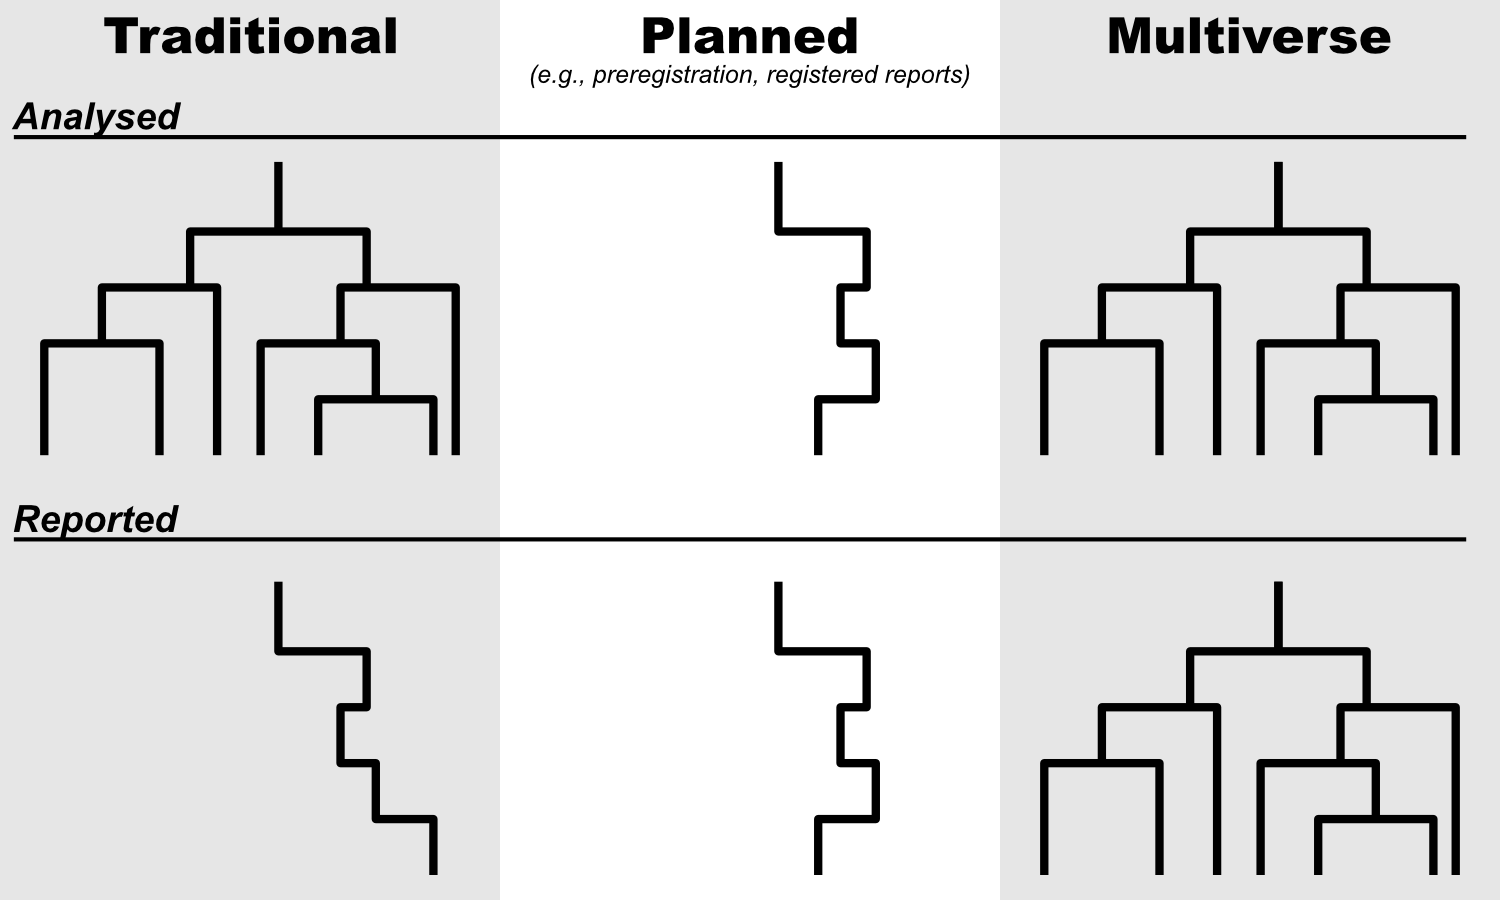
\includegraphics[width=1\linewidth]{../ext_images/Multiverse compared diagram} \caption{Diagram showing how multiverse analysis differs from other approaches. Each branch node represents a choice made during aysnalis}\label{fig:multiDiagram}
\end{figure}

Ecological systems are complex to study and frustrate replication efforts (\protect\hyperlink{ref-nakagawa_replicating_2015}{Nakagawa \& Parker, 2015}; \protect\hyperlink{ref-schnitzer_would_2016}{Schnitzer \& Carson, 2016}), and in the case of movement ecology, the data analysed (i.e., derived data, such as step length, speed, and turn angle derived from timestamped coordinate data) require multiple stages of preprocessing.
Therefore, multiverse analysis is an avenue to explore causes of variation between studies without the additional costs of practical studies, while also being capable of exploring data processing decisions that may not have immediately apparent impacts on final results.

If the data entropy (the process in which as data ages the chances of irreversible loss increase, \protect\hyperlink{ref-vines_availability_2014}{Vines et al., 2014}) and resistance to data sharing (\protect\hyperlink{ref-miyakawa_no_2020}{Miyakawa, 2020}; \protect\hyperlink{ref-tedersoo_data_2021}{Tedersoo et al., 2021}) can be overcome, we will be able to retroactively explore the impact of researcher degrees of freedom on ecological studies (\protect\hyperlink{ref-rijnhart_assessing_2021}{Rijnhart et al., 2021}).
Such retroactive assessment is an attractive option when other methods to explore false positive rates (\protect\hyperlink{ref-hoffmann_multiplicity_2021}{Hoffmann et al., 2021}), such as preregistration and registered reports (\protect\hyperlink{ref-kaplan_likelihood_2015}{Kaplan \& Irvin, 2015}; \protect\hyperlink{ref-scheel_excess_2021}{Scheel, Schijen \& Lakens, 2021}), will require more time to yield results.
Ideally we can use multiverse analysis with preregistrations to boost transparency surrounding the inclusion of decisions and the rationale behind others exclusions (\protect\hyperlink{ref-dragicevic_increasing_2019}{Dragicevic et al., 2019}; \protect\hyperlink{ref-simonsohn_specification_2020}{Simonsohn, Simmons \& Nelson, 2020}).
Given the success of meta-analyses to overcome short-comings in the publication record {[}e.g., p-hacking; Head et al. (\protect\hyperlink{ref-head_extent_2015}{2015}){]}, multiverse analysis may aid the direction of future research efforts by providing a means of meeting calls to replicate results before collecting more (\protect\hyperlink{ref-nuijten_verify_2018}{Nuijten et al., 2018}).

However, as not all choices are equally valid, so multiverse analysis cannot simply provide a correct answer (\protect\hyperlink{ref-steegen_increasing_2016}{Steegen et al., 2016}) --the ``average'' result is not necessarily the closest to the truth.
If we were to undertake a multiverse analysis in a scenario with a ``known truth'', i.e., using a simulated dataset (\protect\hyperlink{ref-bastiaansen_time_2020}{Bastiaansen et al., 2020}), we may be able to detect identify the amount of variation from different sources {[}e.g, biological variation vs study design variation; Breznau et al. (\protect\hyperlink{ref-breznau_observing_2021}{2021}){]}, and potentially the systematic biases stemming from specific choices (potentially via Bayesian Causal Forests \protect\hyperlink{ref-bryan_replicator_2019}{Bryan, Yeager \& O'Brien, 2019}).

Use of simulated data is an established way to explore the robustness of methodologies (\protect\hyperlink{ref-minchin_simulation_1987}{Minchin, 1987}; \protect\hyperlink{ref-silva_reptiles_2020}{Silva et al., 2020}); and this project will harness the benefits of simulated data to assess the impacts of researcher degrees of freedom on the results garnered from animal movement datasets via a multiverse approach.

Here we describe the initial plan to undertake a multiverse approach to explore how decisions concerning the design and analysis of an animal tracking study can impact the findings on habitat selection.
We describe the simulated scenarios we plan to base the study upon and a preliminary multiverse branching path consisting of three analysis approaches, as well as several broad hypotheses.

\hypertarget{methods}{%
\section{Methods}\label{methods}}

\hypertarget{simulating-the-scenarios}{%
\subsection{Simulating the Scenarios}\label{simulating-the-scenarios}}

We simulated three scenarios/species, comprising of different animals and landscapes.
We simulated the landscapes using the NLMR v.1.1.1 package (\protect\hyperlink{ref-NLMR}{Sciaini et al., 2018}), and the animal movement using abmAnimalMovement v.0.1.3.0 (\protect\hyperlink{ref-abmAnimalMovement}{Marshall \& Duthie, 2022}).
The abmAnimalMovement simulations are a discrete time, agent-based modelling approach for simulating animal movement.
Further details of how the scenarios were parametrised can be found in (\protect\hyperlink{ref-abmAnimalMovement}{Marshall \& Duthie, 2022}), and also in the abmAnimalMovement github repository (\href{https://github.com/BenMMarshall/abmAnimalMovement/tree/main/notebook/manuscript}{abmAnimalMovement Github}).

In brief:
- Species 1, Badger: site fidelity to two shelter sites, a low movement speed constrained by terrestrial environment and territoriality, an 8-12 hour activity cycle with seasonal shifts.
- Species 2, Vulture: medium site fidelity via the use of multiple roosting/resting sites a high and variable movement speed with minimal landscape resistance, an 8-12 hour activity cycle with seasonal shifts.
- Species 3, King cobra: lower site fidelity making use of many shelter sites, a medium movement speed through a landscape with high resistance barriers, an 8-12 hour activity cycle combined with a approximately weekly forage-digest cycle and a weak seasonal cycle.

Each simulation generated a years worth of movement data, with a data point recorded every minute.

Our landscapes comprise of three elements, which are considered by the animal differently depending on the behavioural state the animal is in (resting, exploring, foraging).
The three elements were matrices where each cell describes either foraging quality, shelter site quality, and movement ease.
The three are non-independent, and based on a single initial random generation using a Gaussian field.

From the initial Gaussian field we altered the values to exaggerate the difference between high resource areas and low value areas.
Broadly, we created: core resource areas (e.g., forests) with higher foraging quality but lower movement ease, edge areas that overlap with the forest with better movement ease, and more barren areas with high movement ease but with minimal foraging value.
All shelter sites occurred within the higher quality core resource areas.

While our landscapes comprise of continuous values that determine the probability of a simulated animal using a cell or not, many habitat selection studies use categorical habitat metrics or land use types.
Therefore, to simply the interpretation of the multiverse we simplify out landscape into three distinct categories for analysis (Fig. \ref{fig:landscapeExample}): a low quality area where resources are low but movement is easy (class 0 in the figure), an edge habitat with middling resources and high movement ease (class 1), and a high resource habitat with low movement ease (class 2).
While the categroisation of landscapes is a major decision during the analysis of habitat preference, we elected to keep the lanscape classification constant to maintain an feasible multiverse analysis.

\begin{figure}

\includegraphics[width=1\linewidth]{../prereg/figures/landscapeExample} \caption{An example of the underlying environmental matricies used during simulation, and the subsequent habitat classes to be used in the habitat selection analysis.}\label{fig:landscapeExample}
\end{figure}

\hypertarget{sampling-and-analysis-options}{%
\subsection{Sampling and Analysis Options}\label{sampling-and-analysis-options}}

Ultimately number of variations and choices we were able to explore is dictated by computational costs and time.
No multiverse can ever be entirely comprehensive, but we endeavoured to include the major decisions that are required during analysis that may not have immediately apparent ``correct'' answers.

\hypertarget{sampling}{%
\subsubsection{Sampling}\label{sampling}}

The first decisions concern data quantity.
We varied tracking duration and tracking frequency primarily, while keep consistency fixed.
While tracking consistency, or random/systematic data loss during tracking, is an element affecting data quantity the numerous ways of defining consistency means we did not explore tracking consistency at this time.
Tracking timing is also an important consideration; for example, recording the locations of a diurnal animal only at night is highly unlikely to be a viable way of determining foraging choices.
For this exploration we assumed that the researcher has sufficient knowledge about the animal's ecology to prioritise tracking during active hours.
Timing only becomes a consideration when tracking frequency lowers to the point where the tracks performed during a day could occur entirely outside the animal's active period.
Therefore, for the lower tracking frequencies we ensured that daily tracking was centred around midday (as all our simulated species had diurnal activity patterns).

Data or location quality is another point of sampling variation.
Different bio-logging equipment, terrain, animal behaviour, and weather can all impact the location error when tracking an animal.
As the causes and measurement of error, as well as the solutions to, location error are numerous we will not be exploring the impact of error during this exploration in favour of more variation in other decision nodes.

In summary, the sampling decisions will cover variation in species, tracking frequency, and tracking duration (Fig. \ref{fig:decisionTrees}A).

\hypertarget{analysis}{%
\subsubsection{Analysis}\label{analysis}}

For the analysis decisions we focused entirely on decisions that result from an R analysis workflow.
R presents the number one tool for analysing animal movement data (\protect\hyperlink{ref-joo_recent_2022}{Joo et al., 2022}).
Joo et al. (\protect\hyperlink{ref-joo_navigating_2020}{2020}) provides a review of the R packages available to analysis movement data in R, and we used this review as a resource for determining the options for habitat analysis.
Specifically, we explored a subset of decisions made during the workflows using adehabitatHS v.0.3.17 (\protect\hyperlink{ref-adehabitatHS}{Calenge \& Mathieu Basille, 2023}), and amt v.0.2.1.0 (\protect\hyperlink{ref-amt}{Signer, Fieberg \& Avgar, 2019}) R packages.
During the writing of this paper, a new method was described as part of the ctmm package v.1.1.1 (\protect\hyperlink{ref-ctmm}{Fleming \& Calabrese, 2023}), which we also preliminarily investigate.

Combined the packages offer many options for habitat analysis, we focus on four that tackle individual habitat selection.
One from the adehabitatHS package: resource selection ratios (Wides).
Two from the amt package: resource selection function (RSF), step selection function (SSF)
And the newly described Weighted Resource Selection Function (wRSF \protect\hyperlink{ref-alston_mitigating_2023}{Alston et al., 2023}) from the ctmm package.
Each of the methods require downstream decisions resulting in a ``garden of forking paths'' to a final estimate of habitat selection (Fig. \ref{fig:decisionTrees}B).

The Wides and RSF methods share many analysis decisions, principally concerned with how available habitat is defined.
The first decisions is whether to approach the habitat selection analysis as a type I, II or III design, as we are concerned about an individuals' habitat selection we will ignore type I.
While type II habitat selection can identify individual preference, it requires habitat availability to be defined on a population or landscape scale (i.e., a universal availability).
As movement data presents an opportunity to estimate individual preference, and we are not simulating a true interacting population, we focus on type III.
Type III and the need to individually define available habitat opens up many different analytically decisions concerning how that availability is defined.

We used a range of methods are build areas from the recorded locations of the animal: Minimum convex polygons (MCPs), Kernel Density Estimations (KDEs), Autocorrelated Kernel Density Estimations (AKDEs), and dynamic Brownian Bridge Movement Models (dBBMMs).
Minimum convex polygons (MCPs) simply creates a polygon based on the out most locations, where the interior angles sum to less than 180 degrees.

Kernel Density Estimations (KDEs) use kernel smoothing to build a heat map of use or utilisation.
Critical to KDEs operation is a bandwidth or smoothing factor (h) that alters the resulting area treated as used by the animal (\protect\hyperlink{ref-silva_reptiles_2020}{Silva et al., 2020}).
For this analysis we use the the reference bandwidth (href) as it is commonly used (\protect\hyperlink{ref-crane_lots_2020}{Crane et al., 2020}), while also quickly and consistently calculable on a individual by individual basis.
An alternative common method to determine smoothing factor is Least Squares Cross Validation (LSCV).
However, we avoided the LSCV method for two reasons: 1) the LSCV method can fail to converge on a smoothing factor thereby introducing an unpredictable fail state in any potential multiverse, 2) the more limited area estimate it produces make it less suitable for defining habitat availability.

The limitations of MCPs and KDEs have prompted the development of newer methods of area use estimation (\protect\hyperlink{ref-silva_reptiles_2020}{Silva et al., 2020}) that better account for the non-independence and autocorrelative structures within animal movement data (\protect\hyperlink{ref-Noonan2018}{Noonan et al., 2019}).
We used two of these methods to define availability.

First is the Autocorrelated Kernel Density Estimations (AKDEs) (\protect\hyperlink{ref-Fleming2015}{Fleming et al., 2015}; \protect\hyperlink{ref-Fleming2017}{Fleming \& Calabrese, 2017}) from the ctmm package (\protect\hyperlink{ref-Calabrese2016}{Calabrese, Fleming \& Gurarie, 2016}; \protect\hyperlink{ref-ctmm}{Fleming \& Calabrese, 2023}).
The ctmm package provides a workflow for creating an area estimate based on a number of movement models.
The movement models include different levels of autocorrelative structure: Ornstein-Uhlenbeck (OU) models account for central tendency, the Ornstein--Uhlenbeck Foraging (OUF) build on this by also accounting for autocorrelation in movement speed, while the Independent Identically Distributed (IID) models assume location independence meaning they are similar to traditional kernel density approaches.
Each model type is also fitted in isotropic (circular) or anisotropic (elliptical) forms.
The movement model used would constitute a decision during analysis; however, the ctmm package allows for model comparisons (using AICc) to chose a single best model.
Therefore, we use the guidance from (\protect\hyperlink{ref-silva_autocorrelationinformed_2022}{Silva et al., 2022}) to generate weighted AKDEs using perturbative hybrid residual maximum likelihood method (pHREML), and select the best performing by AICc for inclusion in further analysis.
Using weighted AKDEs means the area estimates better address gaps between locations (\protect\hyperlink{ref-silva_autocorrelationinformed_2022}{Silva et al., 2022}), with no apparent drawbacks nor large computational cost.

The second movement-specific method we used was dynamic Brownian Bridge Movement Models (dBBMMs) (\protect\hyperlink{ref-Kranstauber2012}{Kranstauber et al., 2012}) from the move package (\protect\hyperlink{ref-move}{Kranstauber, Smolla \& Scharf, 2023}), which estimates movement capacity of the animal to calibrate repeated random walks between known locations.
DBBMMs require a window and margin size that defines the number of data points over which movement capacity (motion variance) is calculated (\protect\hyperlink{ref-Kranstauber2012}{Kranstauber et al., 2012}).
Window and margin are defined by a number of data points; therefore, to keep the time they represent the same between different tracking frequencies, we changed their values for each tracking frequency.
As our most infrequent tracking is 168 hours (1 week), we set the window to the number of data points collected over 168 hours, and a margin of 48 hours.
The broader window and margin sizes helped reduce computational costs, a major concern when so many dBBMMs are being calculated.

Unlike the AKDEs, dBBMMs do not produce an utilisation distribution.
As dBBMMs are estimating the uncertainty surrounding potential movement pathways, the resulting distribution is better described as an occurrence distribution.
This occurrence distribution is describing the within-sample uncertainty rather than the potential areas available to the animal beyond the sampling period (i.e., it possess little to no predictive capabilities).
Therefore, using dBBMMs to define habitat availability means rather than comparing the habitat use (derived from the movement data) to availability (broader area predicted by the movement data), we are more closely comparing comparing habitat use to an alternative measure of habitat use.
We included dBBMMs to examine whether this arguably easy-to-make conceptual mistake impacts the final results.

What is considered available to an animal is not cleanly translated from biological concept to a statistical one.
While the area estimation methods (MCPs, KDEs, AKDEs, dBBMMs) described above make --to varying degrees-- use of the movement information contained within the dataset they remain abstractions of the underlying drivers of animal movement (i.e., selection and perception).
Therefore, the researcher must make a some-what arbitrary choice regarding what is included/excluded and counted as available; Each of these area estimation methods require a choice to be made regarding the outermost boundary.
We explored the impact of using a 90, 95, and 99\% contour for all the methods.
MCPs areas are generated based a percentage of the location points.
Whereas the KDE, AKDE, and dBBMM methods require a contour to be extracted from the utilisation distribution (occurrence distribution for dBBMMs).
AKDEs also provide a 95\% confidence interval surrounding any chosen contour; for the purposes of simplicity we only use the point estimate for each \% contour.

Once we had created a defined availability area, we generated points at which the habitat type is recorded to estimate the relative availability.
How many and in what alignment these availability points are generated poses two additional points of analytical choice.
For this study we varied the number of availability points as a multiple of the number of animal locations in the dataset: {[}ADD IN R CODE TO PULL THE CHOICE FROM THE TARGETS SCRIPT{]}.
For the alignment of the points, points where either random or stratified within the available previously defined.

As mentioned resource selection function (RSF) share the above decisions on availability with the Wides methods.
In addition, for the RSF we also explored the impact of varying the weighting of the available points when the RSF (i.e., generalized linear model / logistic regression) model is run, which impacts the fitting process.
There are suggestions that altering the weighing can improve model convergence and decrease the uncertainty surrounding habitat preference estimates (\protect\hyperlink{ref-fieberg_how_2021}{Fieberg et al., 2021}); we included this decision to examine whether the pursuit of a more confident answer is biasing the point estimate.

Other than the area based methods of Wides and RSF, we also explored of Step Selection Functions (SSF) and Weighted Resource Selection Functions (wRSF).

Instead of estimating habitat availability using area, SSFs use observed step lengths and turn angles to generate available locations at each time step (i.e., for each data point in the dataset; strata).
As a result SSFs have a number of decisions not shared with the area methods.

We explored three decisions associated with the generation of random (available but unused) locations for each step.
The first is similar to the area methods, we varied the number of random locations generated per step from \#\# to \#\#.
The second and third are concerning the distributions used to generate the random step and turn angles.
Step lengths were tested with a Gamma and Exponential distributions, while turn angle was tested with Von-Mises and Uniform distributions.

The other decisions we explored in SSFs was whether to run the model as a standard step selection or an integrated step selection function.
The standard step selection model is a conditional logistic regression, where we aim to estimate the used/non-used by the habitat values (case\_ \textasciitilde{} values + strata(step\_id\_)).
The integrated step selection model is very similar, apart from the predictors also included step length and turn angle.
The addition of these two components is meant to reduce bias by better accounting for the selection that may simply be an artefact of the movements of the animal rather than active habitat preference (\protect\hyperlink{ref-avgar_integrated_2016}{Avgar et al., 2016}).

We have neglected to explore an expansive aspect of SSFs regarding high resolution data and the use of ``bursts''.
Bursts are used when the researcher wants to look at selection at a given timeframe; therefore. locations are grouped into bursts and the bursts become the strata in the model rather than timestep.
Such grouping of data deserves investigation, but the myriad of ways bursts can be defined and their interaction with tracking duration, frequency, and consistency would warrant a separate multiverse analysis.
As such we have restricted this exploration to step selection functions where the datapoints are equal to the strata in the model.

Compared to the other methods, Weighted Resource Selection Functions do not have many associated choices.
Part of the motivation behind their development was to integrate autocorrelation and other critical structures of movement data into the modelling of habitat preference (\protect\hyperlink{ref-alston_mitigating_2023}{Alston et al., 2023}).
This contrasts to the other methods that either ignore the confounding effect of these structures, or rely on --potentially arbitrary-- decisions with regards to how to mitigate any biasing effects the structures produce.
As a result we have no exploration of analysis decisions for this method because aspects such an available area or points not longer apply, and availability is estimated as part of the model (\protect\hyperlink{ref-alston_mitigating_2023}{Alston et al., 2023}).
Instead we exploring only variations in data quantity (i.e., tracking duration and frequency).

\hypertarget{assessing-the-multiverse}{%
\subsection{Assessing the multiverse}\label{assessing-the-multiverse}}

To generate the multiverse we used a meta-programming approach via the targets v.1.1.2 and tarchetypes v.0.7.6 R packages (\protect\hyperlink{ref-targets}{Landau, 2021a},b).
The targets package was created to facilitate reproducible workflows, but is also paired with functionality enabling multiple analysis routes and parallel processing.
Targets' ability to track analysis task progress and intermediate R objects reduces repeat computation a complex workflow may not be able to be run in a single sitting.
We created a branching analysis workflow based on the decisions we wished to explore, then used targets to iterate over all combinations of all decisions and compile all analysis end points ready for further examination.

Further examination was complicated by the three methods described above producing habitat preference values on different scales with different decisions associated with them.
We elected to analyse the impact of the decisions separately.
For each method we ran two Bayesian regression models to explore: 1) which decisions best explain the absolute deviation from the median estimated preference, 2) which decisions best explain the transformed deviation from the median estimated preference.
The first model provides us with an idea of the decisions that can lead to random, but potentially unbiased noise surrounding the median estimate; whereas the second model highlights decisions that lead to systematic over or under estimation of a habitat preference.

We elected to have the model try and predict the median estimate of habitat preference because the simulation cannot provide a direct analogous value to the outputs of all three methods.
Although the simulation is a discrete time model, where the animal makes decisions based upon a number of options, is similar to a step selection model, the decision making of the animal is made on two time frames breaking our ability to directly compare simulation values with step selection outputs.
Further, the simulated preference of the animal is balanced against other demands such as site fidelity, movement resistance, and avoidance of certain locations.
The closest analogous values we could generate came from running RSF and iSSF models directly on the simulated decisions made by the animal.
We ran these models for both time scales: movement decisions every time step, and destination decisions every behavioural state switch.
These model results, while not strictly comparable to the other outputs, help confirm the animal was correctly preferring the chosen habitat (bare in mind the animal had a no preference exploratory state that would weaken the effect), and support the use of the median estimate to explore the cause behind the most deviant estimates.

We assessed Bayesian model convergence using rhat values, acf, and trace plots.
Based on these assessments we modified the running parameters {[}FINAL VALUES HERE{]}

\hypertarget{results}{%
\section{Results}\label{results}}

The completion of the multiverse resulted in 594 datasets representing an individual animals movements sampled via a distinct tracking regime (i.e., a combination of tracking frequency and duration).
The datasets covered 3 virtual species, 4 individuals per species, frequencies from 0.006 to 2 locations per hour, and durations from 7 to 240 days.
Each of these datasets underwent every combination of analysis choices resulting in
281,952 estimates of habitat preference (Wides: 38,016 , RSF: 228,096 , SSF: 15,840).

\hypertarget{general-patterns}{%
\subsection{General patterns}\label{general-patterns}}

We can get an initial impression of the pattern of the final estimates of preference using a specification curve .
In a scenario where the decisions make little difference, all estimates should group together around a common answer, with the majority of deviation from that common answer the result of sampling or individual variation.

Starting with the Wides results, we see a quite gentle \emph{S} shape {[}FIGURE LINK HERE{]}, with most estimates falling in the range of 0.5 to 2.
While there is a clear agreement of positive selection for habitat 2 as expected, the exact estimate appears relatively sensitive to the choices made.
Looking at the specific choices, we can see several weak patterns.
The first is in tracking duration where we see slight reduction in the spread of estimates with longer tracking durations.
The same is not clear in tracking frequency, because the lower tracking frequency could not be combined with lower tracking durations, resulting in fewer estimates for low frequency scenarios.
Despite this, we do see a slight reduction in estimate variation from frequencies of 0.17 locations per hour and higher.
Similar to the tracking intensity choices, the contour used during the area generation appears to affect the spread of estimates, with a larger contour leading to a greater agreement between estimates.
So to does the multiplier of available points, with more points slightly reducing the spread of estimates, although we see no movement in the median estimate.
Higher numbers of available points, and a higher tracking intensity did appear to lead to a greater chance of a successful estimate being produced (see numbers to the left of the 0 line in {[}LINK TO FIGURE{]}).
The choice of area method (MCP = Minimum Convex Polygon, AKDE = Autocorrelated Kernel Density Estimate based on the best performing movement model, KDEhref = Kernel Density Estimate using reference bandwidth selection, dBBMM = dynamic Brownian Bridge Movement Model) appears to suggest more consistently similar estimates with AKDE and KDEhref methods compared to MCPs and dBBMMs, with MCPs potentially leading to lower estimates in general.

The Resource Selection Function (RSF) specification curve shows a more ideal \emph{S} shape, with the majority of estimates clearly converging on a common answer {[}FIGURE LINK HERE{]}.
Similar to the Wides analysis the majority of the answers, and medians detected preference for habitat 2; and while there are answers suggesting avoidance of habitat 2, all bar two medians connected to a specific choice (the lowest two tracking frequencies) suggest preference.
To best see the changes in variation connected to a given choice, we can look at the rates and position of the outliers (highlighted in purple and orange).
Although weak patterns, tracking duration, frequency, and multiplier of available points see slight reductions in the number of estimates very high or very low.
Other patterns are difficult to discern, except for the weighting of used points that has a clear impact on the outlying low estimates.
The distinct step-like pattern is a result of the logarithmic scale the weighting varies over (required to capture such a wide range of possible values), which can been seen reflected in other choices' groupings of estimates.
Overall the weighting does not appear to impact the overall median, with weighting only appearing to dramatically impact the outlying results.

For the RSF analyses we also recovered the range of the 95\% confidence intervals surrounding each estimate.
When plotted against the estimate we see a clear groupings where those most extreme estimates are also, by a significant margin, the most uncertain.

The Step Selection Function (SSF) specification curves appears even more successful than the RSF.
There is a decently clear \emph{S} shape indicating many analysis end points resulting in similar estimates of preference.
There are also considerably fewer estimates that indicate avoidance of habitat 2.
The stand out patterns are more easily seen in the outlying high estimates.
Once again there are indications of fewer outlying high estimates when data quantity increases, both with duration and frequency.
The number of points per step (or strata) appears to intuitively follow that more available steps leads to more consistent estimations, and also the outliers that exist appear to become less extreme.
The decisions concerning the distributions used to model step lengths and turn angles, as well as whether the model is integrated or not appear to make little difference to the final estimates.

Very much like the RSF explorations of the raw data, the 95\% confidence intervals are dramatically larger (between 100 and 1000 fold) for the outlying estimates than those nearer the median estimate.

The Weighted Resource Selection Function approach has very few decisions associated with it currently; however, we still explored the impact of tracking duration and frequency on the estimates.
The highest estimates appear connected to the lower tracking frequencies, but like the SSF results those high estimates also tend to have large confidence intervals.
The bulk of the estimates agree and are tightly concentrated around the median with very few underestimating.

\hypertarget{model-exploration}{%
\subsection{Model exploration}\label{model-exploration}}

While the specification curves are a good way of getting an intuitive sense of variation, the scale and range of estimates can skew ones' interpretation of which choices have the largest impact.
Our Bayesian models cut through the noise displayed in {[}FIGURES XXXXXXX{]} to reveal more generalised patterns and absorb variation stemming from the stochastic nature of the animal simulations (i.e., variation between individuals and species).

For the decisions connected to Wides results, the absolute deviation was curtailed most effectively by increases in data quantity, with increases in tracking duration (\(\beta\) -0.014, 95\% median Highest-Density Continuous Interval CrI -0.016 -- -0.011) being marginally more effective than tracking frequency (\(\beta\) -0.008, 95\% CrI -0.011 -- -0.006).
Of the other decisions only the multiplier of available points appeared to decrease absolute deviation unambiguously (\(\beta\) -0.003, 95\% CrI -0.004 -- -0.002), and it's effect was much smaller than those concerning data quantity.
Choice of area method as well as the pattern used to generate random points seem to make little clear difference, with all credible intervals connected to those choices overlapping zero.
Contour choice increases the absolute deviation from the median estimate \(\beta\) 0.007, 95\% CrI 0.006 -- 0.008, that appears counter to the initial specification curve plot and highlights the difficulty of identifying patterns from the raw data alone.

The model examining raw deviation from the median estimate reveals that the Wides approach is contrastingly impacted by tracking frequency \(\beta\) 0.039, 95\% CrI 0.036 -- 0.042 and tracking duration \(\beta\) -0.054, 95\% CrI -0.057 -- -0.051, with the former leading to greater estimates of preference.
The impact of stratified versus random available point positioning \(\beta\) -0.001, 95\% CrI -0.004 -- 0.002 and the available points multiplier \(\beta\) -0.003, 95\% CrI -0.004 -- -0.001 have little impact mirror the lack of impact in the absolute deviation model.
All area related choices do not move relative to each other, and reveal that MCPs as an area method to to lead to lower estimates of preference in this scenario, mirroring the lower median displayed in {[}FIGURE XX{]}.

Every decision examined by the RSF absolute effect model appears to be make a difference when estimating preference.
Like the Wides analysis, data quantity is most important.
The two largest effects are from tracking duration (\(\beta\) -0.819, 95\% CrI -0.863 -- -0.779) and frequency (\(\beta\) -1.499, 95\% CrI -1.536 -- -1.458), showing that more data leads to more stable estimates of habitat preference (i.e., more likely to get an answer closer to the overall median estimate).

However, unlike with Wides the other analysis decisions also matter, although to varying extents.
It appears that larger contours (\(\beta\) -0.253, 95\% CrI -0.272 -- -0.233) and a greater multiplier of available points (\(\beta\) -0.239, 95\% CrI -0.258 -- -0.218) decreases the deviation from the median estimate.
To a small extent using a stratified available points pattern lead to lower deviation from the median than a purely random available points pattern (\(\beta\) -0.059, 95\% CrI -0.1 -- -0.019).
Choice of area method can alter results in two ways.
Compared to using MCPs both AKDE (\(\beta\) -0.236, 95\% CrI -0.292 -- -0.18) and KDEhref (\(\beta\) -0.249, 95\% CrI -0.301 -- -0.192) produce estimates more likely to be closer to the median estimate, and to similar degrees.
Dynamic Brownian Bridge Movement Models on the other hand are more likely to lead to greater variation in estimates than those analyses that use MCPs (\(\beta\) 0.307, 95\% CrI 0.249 -- 0.364).

Examining the interactions between tracking duration and frequency with the area methods further reveals the connection between dBBMMs are more variable estimates.
While the other area methods interact with tracking duration in a similar fashion, dBBMMs are more sensitive meaning that at shorter tracking durations the variation created by choosing dBBMMs over another method is greater.
When interacting with tracking frequency the sensitivity is less pronounced, instead we see MCPs being the most sensitive to a lowering of tracking frequency.

The RSF model examining raw deviation from the median estimate reveals a general tendency for higher data quantity to leading to more conservative estimates of preference (tracking duration \(\beta\) -0.429, 95\% CrI -0.479 -- -0.387 and tracking frequency \(\beta\) -0.149, 95\% CrI -0.195 -- -0.102).
While the simulation parametrisation makes it impossible to definitively determine whether this conservatism is correct, the direct estimates from the simulations using an RSF approach suggest the low positive estimates (also near the median ) are more likely to be the correct estimation of simulated preference via RSF.
This matches the absolute deviation model where more data leads to less deviant estimations.

Stratified available point sampling was associated with more positive estimates of preference (\(\beta\) 0.114, 95\% CrI 0.071 -- 0.159), but also those closer to the median (as indicated by the previous model).
This suggests that random point sampling, by contrast, leads to more variable estimates that tend to be lower.
The same pattern is visible in available points multiplier, where more points lead to a more consistent estimate but with a tendency for that estimate to be higher (\(\beta\) 0.527, 95\% CrI 0.504 -- 0.55).

The area method choices reveal a similar pattern.
Dynamic Brownian Bridge Movement models were connected to the more variable estimates, but this model reveals that the variability did not tend towards a particular direction (\(\beta\) -0.047, 95\% CrI -0.107 -- 0.019).
Whereas the other methods are connected to lower deviation from the median estimate, but higher raw estimates.
The area contour selected also reflects this (\(\beta\) 0.538, 95\% CrI 0.515 -- 0.563).
Taken together it appears methods that capture a spatially broader picture of availability have a tendency to produce more stable (in relation to other analysis decisions) but higher estimates of preference.
The dBBMMs by contrast are more vulnerable to variation in other decisions, a trait reflected in the interaction with data quantity measures.

Overall there does not appear to be a decision that leads to great deviation from the median estimate in one direction.

The SSF absolute deviation model matches very closely the previous two models, with tracking quantity both in terms of duration (\(\beta\) -1.471, 95\% CrI -1.552 -- -1.398) and frequency (\(\beta\) -1.676, 95\% CrI -1.758 -- -1.6) dominate in regards to the explaining why estimates tend to be closer to the median estimate.
Unlike the other analysis all other decisions made negligible impact to an estimate's absolute proximity to the median estimate.

Due to the one sided variability of the SSF estimates the raw deviation model mirrors the absolute deviations almost exactly.
The only noticeable difference is in the step distribution decision that changes the direction of the beta point estimate from negative to positive (\(\beta\) 0.015, 95\% CrI -0.144 -- 0.186).
However, the large overlap with zero means that in both cases the step distribution decision is not making a considerable impact to the estimates relative to the median estimate.

The results from the WRSF models are largely similar to the SSF models, although with fewer decisions.
Both tracking duration and tracking frequency lead to lower deviation from the median estimate (tracking duration \(\beta\) -0.321, 95\% CrI -0.474 -- -0.172 and tracking frequency \(\beta\) -0.404, 95\% CrI -0.569 -- -0.25), and the nearly exclusively positively skewed outliers mean that lower raw deviation is associated with lower estimates (tracking duration \(\beta\) -0.321, 95\% CrI -0.474 -- -0.172 and tracking frequency \(\beta\) -0.232, 95\% CrI -0.418 -- -0.072).
The only difference, although both effects overlap considerably, is that increased tracking duration tended to be linked more strongly with lower preference estimates, whereas increased tracking frequency was more connected to less variable estimates in absolute terms.

\hypertarget{discussion}{%
\section{Discussion}\label{discussion}}

Our multiverse exploration of individual habitat selection analysis methods reveals the importance of data quantity in generating consistent results.
Regardless of the approach used, data quantity resulted in estimates of habitat preference closer to the median estimate and more consistently in line with the underlying simulated habitat selection.
There appeared to be an reduction in deviation from the median estimate when using newer methods (e.g., SSF and wRSF).
This suggests that advancements in habitat selection analysis methods are not only worthwhile, but actively counter reproducibility issues that may stem from research choice.

The overall pattern in estimates mirror those seen in other fields, where the bulk of answers converge but outliers remain (\protect\hyperlink{ref-silberzahn_many_2018}{Silberzahn et al., 2018}; \protect\hyperlink{ref-simonsohn_specification_2020}{Simonsohn, Simmons \& Nelson, 2020}).
While the incentives for findings positive results remain in the publishing system (\protect\hyperlink{ref-fanelli_positive_2010}{Fanelli, 2010b}, \protect\hyperlink{ref-fanelli_negative_2012}{2012}), using analysis choices to game or mine for a given exciting result appears time consuming because the proportion of the extreme estimates is relatively low compared to the majority of estimates that agree near the median.
Therefore, we can be as confident in past studies findings as we would those from.
If the past habitat preference studies report extreme findings there is a general tendency for these to be paired with very wide confidence intervals; if the studies have reported the confidence intervals, this provides an additional safeguard against over interpretation of potentially incorrect extreme results.

While the goal of this study was not to review and provide direct guidance to the most effective ways of undertaking habitat selection, our findings show several key patterns that fit into previous guidance in the literature.
In particular the benefits of larger datasets and the importance of defining availability (\protect\hyperlink{ref-northrup_practical_2013}{Northrup et al., 2013}; \protect\hyperlink{ref-street_solving_2021}{Street et al., 2021}), latter particularly key because of the potential for subjective definitions (\protect\hyperlink{ref-beyer_interpretation_2010}{Beyer et al., 2010}).
One specific example would be the tendency for larger area methods, and wider contours leading to more stable (nearer the median) estimates; this mirrors previously reveals patterns connecting broader spatial scales and transferability (\protect\hyperlink{ref-paton_defining_2015}{Paton \& Matthiopoulos, 2015}).

The overall pattern shows data quality supremacy, but this cannot be used as an excuse to ignore the decisions during analysis.
Two aspect of the results highlight that complacency is unwise.
First RSF, SSF, and wRSF approaches appear to be more consistent than the more basic and older Wides ratio based approach.
Both RSF, SSF, and wRSF have improved capacity for accounting for the peculiarities movement data structure (e.g., via random effects) than the Wides approach.
Second is the evidence for conceptual mistakes to have impacts on final results, implying that in some cases there are more correct answers to certain analysis decisions.
The use of dBBMMs to define availability is not strictly correct as the (confidence) area generated by dBBMMs are reflected of uncertainty surrounding use.
This renders the down stream analysis of habitat preference a comparison of use (measured by points) to use (measured by area of uncertainty surrounding movement trajectories); as opposed to the desired use versus availability.
The dBBMM results exemplify the need to maintain a connection between abstractions (e.g., an area) of the data and the intended use.
A similar argument can be made for data quantity, where mismatches between frequency and desired behaviours or and inadequate duration will obscure answers regardless of the analysis applied.
Our simulations are diurnal and the tracking spacing was skewed towards those diurnal hours for lower tracking frequency regimes.
Failure to do this, instead allowing locations to be recorded equally at night and day, would have skewed estimates towards the habitat used for shelter rather than foraging.
Matching question to analysis approach remains important, but the cost of mistakes may be less dramatic than feared.

Further good news is that some decisions that are connected to more stable estimates have very little reason not to be maximised.
For example, the points multiplier or points per step decision can be maximised to whatever extent allowed by the computational resources available to the researcher.
Increases in the number of available points will improve the accuracy when defining available habitats; (\protect\hyperlink{ref-street_solving_2021}{Street et al., 2021}), indicates that the systematic sampling with high numbers of points is preferable to capture a complete unbiased availability.
(\protect\hyperlink{ref-fieberg_how_2021}{Fieberg et al., 2021}) states that available points should be high enough to ensure stable coefficient estimates, that is also aided by increased weighting of available points in the logistic regression.
While we did not see the improvements in points per step in the SSF analysis, the benefits of high available steps is more pronounced when working with rare habitat types (\protect\hyperlink{ref-thurfjell_applications_2014}{Thurfjell, Ciuti \& Boyce, 2014}).
More available points reduces the chances of missing small areas of rare habitat; our analysis would not have revealed this because of the abundance of the preferred habitat type.

We did not see large improvements using different step or turn angle distributions, this has been shown to play an increasingly important role in mitigating biased estimates in scenarios with stronger selection strengths (\protect\hyperlink{ref-forester_accounting_2009}{Forester, Im \& Rathouz, 2009}).
The limited cost of integrating step and turn into SSF formula would suggest iSSF formulation is likely always preferable.

\hypertarget{limitations-of-the-multiverse-approach-and-future-directions}{%
\subsection{Limitations of the multiverse approach and future directions}\label{limitations-of-the-multiverse-approach-and-future-directions}}

Study does helps demonstrate the impact of researcher choice in habitat selection studies; the true number of choices is impractical to explore and ever growing.
Time and computational limits compound with the infinite granularity of decision connected to continuous variables (e.g., tracking frequency) to ensure that all choices cannot be completely explored.

The relationship between tracking regime, the data quantity produced, and the resulting habitat selection results is a complex area to assess.
We focused on systematic controlled changes to tracking frequency, but in field scenarios data quantity can be impacted by practical and logistical constraints that results in stochastic data loss.
Newer methods help alleviate the problems with inconsistent tracking (\protect\hyperlink{ref-fleming_correcting_2018}{Fleming et al., 2018}; \protect\hyperlink{ref-silva_autocorrelationinformed_2022}{Silva et al., 2022}; \protect\hyperlink{ref-alston_mitigating_2023}{Alston et al., 2023}), providing an additional reason why analysis decisions should not be ignored.

Ultimately the multiverse approach cannot reveal the true answer; the multiverse's mean result describes the mean of the analysis pathways and does not necessarily converge towards a true effect.
We attempted to make our findings more generalisable by simulating three distinct animal species that move in different fashions and that face differing level of habitat connectivity.
We cannot discount scenarios with different movement characteristics that interact with particular analysis choices to bias habitat selection estimates --scale remains a key consideration for any study (\protect\hyperlink{ref-thurfjell_applications_2014}{Thurfjell, Ciuti \& Boyce, 2014}; \protect\hyperlink{ref-northrup_conceptual_2022}{Northrup et al., 2022}), and context-specific selection remains difficult to translate (\protect\hyperlink{ref-avgar_habitat_2020}{Avgar, Betini \& Fryxell, 2020}).
The difficulty in generalising a ``one-size fits all'' approach highlights the benefits of methods that can be parametrised by the underlying characteristics of the data (e.g., wRSF (\protect\hyperlink{ref-alston_mitigating_2023}{Alston et al., 2023})), and where the uncertainty stemming from sampling can be carried forward to the final estimates.

Despite the inherit limitations of multiverses, the exploration of analysis choice presents an important consideration for any researcher looking to know the reliability of their findings.
More formal and mathematically based estimates of reliability are available for specific approaches, for example RSFs (\protect\hyperlink{ref-street_solving_2021}{Street et al., 2021}), and these present an important component when reporting RSFs.
However, they still require some level of \emph{a priori} decision making (e.g., landscape and availability definition) (\protect\hyperlink{ref-northrup_conceptual_2022}{Northrup et al., 2022}); therefore, researcher choice remains.

Beyond the aforementioned limitations to the multiverse approach there is scope to expand the exploration.
Our next step is to reapply the same meta-programming pipeline approach to population targeting habitat analyses.
A focus on these approaches will allows us to explore the third key component of data quantity --sample size-- as well as how well analyses tackle individual variability either in the analysis itself or during summarising of individual habitat preference estimates.
There are already methods for assessing require sample size to detected a given selection for RSFs (\protect\hyperlink{ref-street_solving_2021}{Street et al., 2021}).

\hypertarget{conclusions}{%
\subsection{Conclusions}\label{conclusions}}

We show, using a multiverse of analysis pathways, that data quantity is an important safeguard against extreme outlying results in individual habitat preference analyses.
The indications that analysis choices are less important than data quantity improves our confidence in previously published habitat preference studies as there is no more scope to mine a desired result than in other disciplines.
Newer methods of habitat preference analysis appear to reduce variation from researcher choice further, indicating that future studies are more likely to be robust that those before.

\hypertarget{acknowledgements}{%
\section{Acknowledgements}\label{acknowledgements}}

\hypertarget{software-availablity}{%
\section{Software availablity}\label{software-availablity}}

In addition to packages already mentioned in the methods we also used the following.

We used \emph{R} v.4.3.0 (\protect\hyperlink{ref-base}{R Core Team, 2023}) via \emph{RStudio} v.2022.7.2.576 (\protect\hyperlink{ref-rstudio}{RStudio Team, 2022}).
We used \emph{here} v.1.0.1 (\protect\hyperlink{ref-here}{Müller, 2020}) and \emph{qs} v.0.25.5 (\protect\hyperlink{ref-qs}{Ching, 2023}) to manage directory addresses and saved objects.

We used \emph{raster} v.3.6.20 (\protect\hyperlink{ref-raster}{Hijmans, 2023}) and \emph{RandomFields} v.3.3.14 (\protect\hyperlink{ref-RandomFields}{Schlather et al., 2015}) to aid landscape raster creation alongside NLMR v.1.1.1 (\protect\hyperlink{ref-NLMR}{Sciaini et al., 2018}).

We used \emph{ggplot2} v.3.4.2 for creating figures (\protect\hyperlink{ref-ggplot2}{Wickham, 2016}), with the expansions: \emph{patchwork} v.1.1.2 (\protect\hyperlink{ref-patchwork}{Pedersen, 2022}), \emph{ggridges} v.0.5.4 (\protect\hyperlink{ref-ggridges}{Wilke, 2022}), and \emph{ggdist} v.3.3.0 (\protect\hyperlink{ref-ggdist}{Kay, 2023a}).

We used \emph{brms} v.2.19.0 (\protect\hyperlink{ref-brms}{Bürkner, 2021}) to run Bayesian models, with dianogistics generated used \emph{bayesplot} v.1.10.0 (\protect\hyperlink{ref-bayesplot}{Gabry et al., 2019}), \emph{tidybayes} v.3.0.4 (\protect\hyperlink{ref-tidybayes}{Kay, 2023b}), and \emph{performance} v.0.10.3 (\protect\hyperlink{ref-performance}{Lüdecke et al., 2021}).

We used the \emph{dplyr} v.1.1.2 (\protect\hyperlink{ref-dplyr}{Wickham et al., 2023}), \emph{tibble} v.3.2.1 (\protect\hyperlink{ref-tibble}{Müller \& Wickham, 2023}), \emph{reshape2} v.1.4.4 (\protect\hyperlink{ref-reshape2}{Wickham, 2007}), and \emph{stringr} v.1.5.0 (\protect\hyperlink{ref-stringr}{Wickham, 2022}) packages for data manipulation.

We used \emph{sp} v.1.6.0 (\protect\hyperlink{ref-sp}{Bivand, Pebesma \& Gomez-Rubio, 2013}), \emph{adehabitatHR} v.0.4.21 (\protect\hyperlink{ref-adehabitatHR}{Calenge \& Scott Fortmann-Roe, 2023}), \emph{move} v.4.1.12 (\protect\hyperlink{ref-move}{Kranstauber, Smolla \& Scharf, 2023}) for manipulation of spatial data and estimation of space use not otherwise mentioned in the methods.

We used rmarkdown v.2.21 (\protect\hyperlink{ref-rmarkdown2018}{Xie, Allaire \& Grolemund, 2018}; \protect\hyperlink{ref-rmarkdown2020}{Xie, Dervieux \& Riederer, 2020}; \protect\hyperlink{ref-rmarkdown2023}{Allaire et al., 2023}), bookdown v.0.34 (\protect\hyperlink{ref-bookdown2016}{Xie, 2016}, \protect\hyperlink{ref-R-bookdown}{2022}), tinytex v.0.45 (\protect\hyperlink{ref-tinytex2019}{Xie, 2019}, \protect\hyperlink{ref-tinytex2023}{2023a}), and knitr v.1.42 (\protect\hyperlink{ref-knitr2014}{Xie, 2014}, \protect\hyperlink{ref-knitr2015}{2015}, \protect\hyperlink{ref-knitr2023}{2023b}) packages to generate type-set outputs.

We generated R package citations with the aid of \emph{grateful} v.0.2.0 (\protect\hyperlink{ref-grateful}{Francisco Rodríguez-Sánchez, Connor P. Jackson \& Shaurita D. Hutchins, 2023}).

Wolen et al. (\protect\hyperlink{ref-osfr}{2020})

We generated R package citations with the aid of grateful v.0.2.0 (\protect\hyperlink{ref-grateful}{Francisco Rodríguez-Sánchez, Connor P. Jackson \& Shaurita D. Hutchins, 2023}).

\hypertarget{data-availabilty}{%
\section{Data availabilty}\label{data-availabilty}}

\hypertarget{references}{%
\section*{References}\label{references}}
\addcontentsline{toc}{section}{References}

\hypertarget{refs}{}
\begin{CSLReferences}{1}{0}
\leavevmode\vadjust pre{\hypertarget{ref-albers_problem_2019}{}}%
Albers C. 2019. The problem with unadjusted multiple and sequential statistical testing. \emph{Nature Communications} 10:1921. DOI: \href{https://doi.org/10.1038/s41467-019-09941-0}{10.1038/s41467-019-09941-0}.

\leavevmode\vadjust pre{\hypertarget{ref-rmarkdown2023}{}}%
Allaire J, Xie Y, Dervieux C, McPherson J, Luraschi J, Ushey K, Atkins A, Wickham H, Cheng J, Chang W, Iannone R. 2023. \emph{\href{https://github.com/rstudio/rmarkdown}{{rmarkdown}: Dynamic documents for r}}.

\leavevmode\vadjust pre{\hypertarget{ref-alston_mitigating_2023}{}}%
Alston JM, Fleming CH, Kays R, Streicher JP, Downs CT, Ramesh T, Reineking B, Calabrese JM. 2023. Mitigating pseudoreplication and bias in resource selection functions with autocorrelation‐informed weighting. \emph{Methods in Ecology and Evolution} 14:643--654. DOI: \href{https://doi.org/10.1111/2041-210X.14025}{10.1111/2041-210X.14025}.

\leavevmode\vadjust pre{\hypertarget{ref-anderson_perverse_2007}{}}%
Anderson MS, Ronning EA, De Vries R, Martinson BC. 2007. The {Perverse} {Effects} of {Competition} on {Scientists}' {Work} and {Relationships}. \emph{Science and Engineering Ethics} 13:437--461. DOI: \href{https://doi.org/10.1007/s11948-007-9042-5}{10.1007/s11948-007-9042-5}.

\leavevmode\vadjust pre{\hypertarget{ref-anvari_replicability_2018}{}}%
Anvari F, Lakens D. 2018. The replicability crisis and public trust in psychological science. \emph{Comprehensive Results in Social Psychology} 3:266--286. DOI: \href{https://doi.org/10.1080/23743603.2019.1684822}{10.1080/23743603.2019.1684822}.

\leavevmode\vadjust pre{\hypertarget{ref-auspurg_has_2021}{}}%
Auspurg K, Brüderl J. 2021. Has the {Credibility} of the {Social} {Sciences} {Been} {Credibly} {Destroyed}? {Reanalyzing} the {``{Many} {Analysts}, {One} {Data} {Set}''} {Project}. \emph{Socius: Sociological Research for a Dynamic World} 7:237802312110244. DOI: \href{https://doi.org/10.1177/23780231211024421}{10.1177/23780231211024421}.

\leavevmode\vadjust pre{\hypertarget{ref-avgar_habitat_2020}{}}%
Avgar T, Betini GS, Fryxell JM. 2020. Habitat selection patterns are density dependent under the ideal free distribution. \emph{Journal of Animal Ecology} 89:2777--2787. DOI: \href{https://doi.org/10.1111/1365-2656.13352}{10.1111/1365-2656.13352}.

\leavevmode\vadjust pre{\hypertarget{ref-avgar_integrated_2016}{}}%
Avgar T, Potts JR, Lewis MA, Boyce MS. 2016. Integrated step selection analysis: Bridging the gap between resource selection and animal movement. \emph{Methods in Ecology and Evolution} 7:619--630. DOI: \href{https://doi.org/10.1111/2041-210X.12528}{10.1111/2041-210X.12528}.

\leavevmode\vadjust pre{\hypertarget{ref-barto_dissemination_2012}{}}%
Barto EK, Rillig MC. 2012. Dissemination biases in ecology: Effect sizes matter more than quality. \emph{Oikos} 121:228--235. DOI: \href{https://doi.org/10.1111/j.1600-0706.2011.19401.x}{10.1111/j.1600-0706.2011.19401.x}.

\leavevmode\vadjust pre{\hypertarget{ref-bastiaansen_time_2020}{}}%
Bastiaansen JA, Kunkels YK, Blaauw FJ, Boker SM, Ceulemans E, Chen M, Chow S-M, Jonge P de, Emerencia AC, Epskamp S, Fisher AJ, Hamaker EL, Kuppens P, Lutz W, Meyer MJ, Moulder R, Oravecz Z, Riese H, Rubel J, Ryan O, Servaas MN, Sjobeck G, Snippe E, Trull TJ, Tschacher W, Veen DC van der, Wichers M, Wood PK, Woods WC, Wright AGC, Albers CJ, Bringmann LF. 2020. Time to get personal? {The} impact of researchers choices on the selection of treatment targets using the experience sampling methodology. \emph{Journal of Psychosomatic Research} 137:110211. DOI: \href{https://doi.org/10.1016/j.jpsychores.2020.110211}{10.1016/j.jpsychores.2020.110211}.

\leavevmode\vadjust pre{\hypertarget{ref-beyer_interpretation_2010}{}}%
Beyer HL, Haydon DT, Morales JM, Frair JL, Hebblewhite M, Mitchell M, Matthiopoulos J. 2010. The interpretation of habitat preference metrics under use--availability designs. \emph{Philosophical Transactions of the Royal Society B: Biological Sciences} 365:2245--2254. DOI: \href{https://doi.org/10.1098/rstb.2010.0083}{10.1098/rstb.2010.0083}.

\leavevmode\vadjust pre{\hypertarget{ref-bishop_rein_2019}{}}%
Bishop D. 2019. Rein in the four horsemen of irreproducibility. \emph{Nature} 568:435--435. DOI: \href{https://doi.org/10.1038/d41586-019-01307-2}{10.1038/d41586-019-01307-2}.

\leavevmode\vadjust pre{\hypertarget{ref-sp}{}}%
Bivand RS, Pebesma E, Gomez-Rubio V. 2013. \emph{\href{https://asdar-book.org/}{Applied spatial data analysis with {R}, second edition}}. Springer, NY.

\leavevmode\vadjust pre{\hypertarget{ref-Brembs2018}{}}%
Brembs B. 2018. Prestigious {Science} {Journals} {Struggle} to {Reach} {Even} {Average} {Reliability}. \emph{Frontiers in Human Neuroscience} 12:1--7. DOI: \href{https://doi.org/10.3389/fnhum.2018.00037}{10.3389/fnhum.2018.00037}.

\leavevmode\vadjust pre{\hypertarget{ref-brembs_reliable_2019}{}}%
Brembs B. 2019. Reliable novelty: {New} should not trump true. \emph{PLOS Biology} 17:e3000117. DOI: \href{https://doi.org/10.1371/journal.pbio.3000117}{10.1371/journal.pbio.3000117}.

\leavevmode\vadjust pre{\hypertarget{ref-breznau_observing_2021}{}}%
Breznau N, Rinke EM, Wuttke A, Adem M, Adriaans J, Alvarez-Benjumea A, Andersen HK, Auer D, Azevedo F, Bahnsen O, Balzer D, Bauer G, Bauer P, Baumann M, Baute S, Benoit V, Bernauer J, Berning C, Berthold A, Bethke FS, Biegert T, Blinzler K, Blumenberg J, Bobzien L, Bohman A, Bol T, Bostic A, Brzozowska Z, Burgdorf K, Burger K, Busch K, Castillo JC, Chan N, Christmann P, Connelly R, Czymara CS, Damian E, Ecker A, Edelmann A, Eger MA, Ellerbrock S, Forke A, Forster AG, Gaasendam C, Gavras K, Gayle V, Gessler T, Gnambs T, Godefroidt A, Grömping M, Groß M, Gruber S, Gummer T, Hadjar A, Heisig JP, Hellmeier S, Heyne S, Hirsch M, Hjerm M, Hochman O, Hövermann A, Hunger S, Hunkler C, Huth N, Ignacz Z, Jacobs L, Jacobsen J, Jaeger B, Jungkunz S, Jungmann N, Kauff M, Kleinert M, Klinger J, Kolb J-P, Kołczyńska M, Kuk JS, Kunißen K, Sinatra DK, Greinert A, Lersch PM, Löbel L-M, Lutscher P, Mader M, Madia JE, Malancu N, Maldonado L, Marahrens H, Martin N, Martinez P, Mayerl J, Mayorga OJ, McManus P, Wagner K, Meeusen C, Meierrieks D, Mellon J, Merhout F, Merk S, Meyer D, Micheli L, Mijs JJB, Moya C, Neunhoeffer M, Nüst D, Nygård O, Ochsenfeld F, Otte G, Pechenkina A, Prosser C, Raes L, Ralston K, Ramos M, Roets A, Rogers J, Ropers G, Samuel R, Sand G, Schachter A, Schaeffer M, Schieferdecker D, Schlueter E, Schmidt K, Schmidt R, Schmidt-Catran A, Schmiedeberg C, Schneider J, Schoonvelde M, Schulte-Cloos J, Schumann S, Schunck R, Schupp J, Seuring J, Silber H, Sleegers WWA, Sonntag N, Staudt A, Steiber N, Steiner N, Sternberg S, Stiers D, Stojmenovska D, Storz N, Striessnig E, Stroppe A-K, Teltemann J, Tibajev A, Tung BB, Vagni G, Van Assche J, Linden M van der, Noll J van der, Van Hootegem A, Vogtenhuber S, Voicu B, Wagemans F, Wehl N, Werner H, Wiernik BM, Winter F, Wolf C, Yamada Y, Zhang N, Ziller C, Zins S, Żółtak T, Nguyen HHV. 2021. Observing {Many} {Researchers} {Using} the {Same} {Data} and {Hypothesis} {Reveals} a {Hidden} {Universe} of {Uncertainty}. \emph{MetaArXiv}. DOI: \href{https://doi.org/10.31222/osf.io/cd5j9}{10.31222/osf.io/cd5j9}.

\leavevmode\vadjust pre{\hypertarget{ref-bryan_replicator_2019}{}}%
Bryan CJ, Yeager DS, O'Brien JM. 2019. Replicator degrees of freedom allow publication of misleading failures to replicate. \emph{Proceedings of the National Academy of Sciences} 116:25535--25545. DOI: \href{https://doi.org/10.1073/pnas.1910951116}{10.1073/pnas.1910951116}.

\leavevmode\vadjust pre{\hypertarget{ref-brms}{}}%
Bürkner P-C. 2021. Bayesian item response modeling in {R} with {brms} and {Stan}. \emph{Journal of Statistical Software} 100:1--54. DOI: \href{https://doi.org/10.18637/jss.v100.i05}{10.18637/jss.v100.i05}.

\leavevmode\vadjust pre{\hypertarget{ref-Calabrese2016}{}}%
Calabrese JM, Fleming CH, Gurarie E. 2016. Ctmm: An {R} {Package} for {Analyzing} {Animal} {Relocation} {Data} {As} a {Continuous}-{Time} {Stochastic} {Process}. \emph{Methods in Ecology and Evolution} 7:1124--1132. DOI: \href{https://doi.org/10.1111/2041-210X.12559}{10.1111/2041-210X.12559}.

\leavevmode\vadjust pre{\hypertarget{ref-adehabitatHS}{}}%
Calenge C, Mathieu Basille contributions from. 2023. \emph{\href{https://CRAN.R-project.org/package=adehabitatHS}{{adehabitatHS}: Analysis of habitat selection by animals}}.

\leavevmode\vadjust pre{\hypertarget{ref-adehabitatHR}{}}%
Calenge C, Scott Fortmann-Roe contributions from. 2023. \emph{\href{https://CRAN.R-project.org/package=adehabitatHR}{{adehabitatHR}: Home range estimation}}.

\leavevmode\vadjust pre{\hypertarget{ref-cassey_survey_2004}{}}%
Cassey P, Ewen JG, Blackburn TM, Møller AP. 2004. A survey of publication bias within evolutionary ecology. \emph{Proceedings of the Royal Society of London. Series B: Biological Sciences} 271. DOI: \href{https://doi.org/10.1098/rsbl.2004.0218}{10.1098/rsbl.2004.0218}.

\leavevmode\vadjust pre{\hypertarget{ref-qs}{}}%
Ching T. 2023. \emph{\href{https://CRAN.R-project.org/package=qs}{{qs}: Quick serialization of r objects}}.

\leavevmode\vadjust pre{\hypertarget{ref-clark_ocean_2020}{}}%
Clark TD, Raby GD, Roche DG, Binning SA, Speers-Roesch B, Jutfelt F, Sundin J. 2020. Ocean acidification does not impair the behaviour of coral reef fishes. \emph{Nature} 577:370--375. DOI: \href{https://doi.org/10.1038/s41586-019-1903-y}{10.1038/s41586-019-1903-y}.

\leavevmode\vadjust pre{\hypertarget{ref-crane_lots_2020}{}}%
Crane M, Silva I, Marshall BM, Strine CT. 2020. Lots of movement, little progress: {A} review of reptile home range literature. \emph{bioRxiv} 2020.12.03.409292. DOI: \href{https://doi.org/10.1101/2020.12.03.409292}{10.1101/2020.12.03.409292}.

\leavevmode\vadjust pre{\hypertarget{ref-del_giudice_travelers_2021}{}}%
Del Giudice M, Gangestad SW. 2021. A {Traveler}'s {Guide} to the {Multiverse}: {Promises}, {Pitfalls}, and a {Framework} for the {Evaluation} of {Analytic} {Decisions}. \emph{Advances in Methods and Practices in Psychological Science} 4:251524592095492. DOI: \href{https://doi.org/10.1177/2515245920954925}{10.1177/2515245920954925}.

\leavevmode\vadjust pre{\hypertarget{ref-desbureaux_subjective_2021}{}}%
Desbureaux S. 2021. Subjective modeling choices and the robustness of impact evaluations in conservation science. \emph{Conservation Biology} 35:1615--1626. DOI: \href{https://doi.org/10.1111/cobi.13728}{10.1111/cobi.13728}.

\leavevmode\vadjust pre{\hypertarget{ref-dragicevic_increasing_2019}{}}%
Dragicevic P, Jansen Y, Sarma A, Kay M, Chevalier F. 2019. Increasing the {Transparency} of {Research} {Papers} with {Explorable} {Multiverse} {Analyses}. In: \emph{Proceedings of the 2019 {CHI} {Conference} on {Human} {Factors} in {Computing} {Systems}}. Glasgow Scotland Uk: ACM, 1--15. DOI: \href{https://doi.org/10.1145/3290605.3300295}{10.1145/3290605.3300295}.

\leavevmode\vadjust pre{\hypertarget{ref-fanelli_positive_2010}{}}%
Fanelli D. 2010b. {``{Positive}''} {Results} {Increase} {Down} the {Hierarchy} of the {Sciences}. \emph{PLoS ONE} 5:e10068. DOI: \href{https://doi.org/10.1371/journal.pone.0010068}{10.1371/journal.pone.0010068}.

\leavevmode\vadjust pre{\hypertarget{ref-fanelli_pressures_2010}{}}%
Fanelli D. 2010a. Do {Pressures} to {Publish} {Increase} {Scientists}' {Bias}? {An} {Empirical} {Support} from {US} {States} {Data}. \emph{PLoS ONE} 5:e10271. DOI: \href{https://doi.org/10.1371/journal.pone.0010271}{10.1371/journal.pone.0010271}.

\leavevmode\vadjust pre{\hypertarget{ref-fanelli_negative_2012}{}}%
Fanelli D. 2012. Negative results are disappearing from most disciplines and countries. \emph{Scientometrics} 90:891--904. DOI: \href{https://doi.org/10.1007/s11192-011-0494-7}{10.1007/s11192-011-0494-7}.

\leavevmode\vadjust pre{\hypertarget{ref-fieberg_how_2021}{}}%
Fieberg J, Signer J, Smith B, Avgar T. 2021. A {``{How} to''} guide for interpreting parameters in habitat‐selection analyses. \emph{Journal of Animal Ecology} 90:1027--1043. DOI: \href{https://doi.org/10.1111/1365-2656.13441}{10.1111/1365-2656.13441}.

\leavevmode\vadjust pre{\hypertarget{ref-Fleming2017}{}}%
Fleming CH, Calabrese JM. 2017. A new kernel density estimator for accurate home-range and species-range area estimation. \emph{Methods in Ecology and Evolution} 8:571--579. DOI: \href{https://doi.org/10.1111/2041-210X.12673}{10.1111/2041-210X.12673}.

\leavevmode\vadjust pre{\hypertarget{ref-ctmm}{}}%
Fleming CH, Calabrese JM. 2023. \emph{{ctmm}: Continuous-time movement modeling}.

\leavevmode\vadjust pre{\hypertarget{ref-Fleming2015}{}}%
Fleming CH, Fagan WF, Mueller T, Olson KA, Leimgruber P, Calabrese JM. 2015. Rigorous home range estimation with movement data: {A} new autocorrelated kernel density estimator. \emph{Ecology} 96:1182--1188.

\leavevmode\vadjust pre{\hypertarget{ref-fleming_correcting_2018}{}}%
Fleming CH, Sheldon D, Fagan WF, Leimgruber P, Mueller T, Nandintsetseg D, Noonan MJ, Olson KA, Setyawan E, Sianipar A, Calabrese JM. 2018. Correcting for missing and irregular data in home-range estimation. \emph{Ecological Applications} 28:1003--1010. DOI: \href{https://doi.org/10.1002/eap.1704}{10.1002/eap.1704}.

\leavevmode\vadjust pre{\hypertarget{ref-forester_accounting_2009}{}}%
Forester JD, Im HK, Rathouz PJ. 2009. Accounting for animal movement in estimation of resource selection functions: Sampling and data analysis. \emph{Ecology} 90:3554--3565. DOI: \href{https://doi.org/10.1890/08-0874.1}{10.1890/08-0874.1}.

\leavevmode\vadjust pre{\hypertarget{ref-forstmeier_cryptic_2011}{}}%
Forstmeier W, Schielzeth H. 2011. Cryptic multiple hypotheses testing in linear models: Overestimated effect sizes and the winner's curse. \emph{Behavioral Ecology and Sociobiology} 65:47--55. DOI: \href{https://doi.org/10.1007/s00265-010-1038-5}{10.1007/s00265-010-1038-5}.

\leavevmode\vadjust pre{\hypertarget{ref-forstmeier_detecting_2017}{}}%
Forstmeier W, Wagenmakers E-J, Parker TH. 2017. Detecting and avoiding likely false-positive findings -- a practical guide: {Avoiding} false-positive findings. \emph{Biological Reviews} 92:1941--1968. DOI: \href{https://doi.org/10.1111/brv.12315}{10.1111/brv.12315}.

\leavevmode\vadjust pre{\hypertarget{ref-grateful}{}}%
Francisco Rodríguez-Sánchez, Connor P. Jackson, Shaurita D. Hutchins. 2023. \emph{\href{https://github.com/Pakillo/grateful}{{grateful}: Facilitate citation of r packages}}.

\leavevmode\vadjust pre{\hypertarget{ref-fraser_role_2020}{}}%
Fraser H, Barnett A, Parker TH, Fidler F. 2020. The role of replication studies in ecology. \emph{Ecology and Evolution} 10:5197--5207. DOI: \href{https://doi.org/10.1002/ece3.6330}{10.1002/ece3.6330}.

\leavevmode\vadjust pre{\hypertarget{ref-fraser_questionable_2018}{}}%
Fraser H, Parker T, Nakagawa S, Barnett A, Fidler F. 2018. Questionable research practices in ecology and evolution. \emph{PLOS ONE} 13:e0200303. DOI: \href{https://doi.org/10.1371/journal.pone.0200303}{10.1371/journal.pone.0200303}.

\leavevmode\vadjust pre{\hypertarget{ref-freedman_economics_2015}{}}%
Freedman LP, Cockburn IM, Simcoe TS. 2015. The {Economics} of {Reproducibility} in {Preclinical} {Research}. \emph{PLOS Biology} 13:e1002165. DOI: \href{https://doi.org/10.1371/journal.pbio.1002165}{10.1371/journal.pbio.1002165}.

\leavevmode\vadjust pre{\hypertarget{ref-bayesplot}{}}%
Gabry J, Simpson D, Vehtari A, Betancourt M, Gelman A. 2019. Visualization in bayesian workflow. \emph{J. R. Stat. Soc. A} 182:389--402. DOI: \href{https://doi.org/10.1111/rssa.12378}{10.1111/rssa.12378}.

\leavevmode\vadjust pre{\hypertarget{ref-gelman_garden_2013}{}}%
Gelman A, Loken E. 2013. \href{http://www.stat.columbia.edu/~gelman/research/unpublished/p_hacking.pdf}{The garden of forking paths: {Why} multiple comparisons can be a problem, even when there is no "fishing expedition" or "p-hacking" and the research hypothesis was posited ahead of time}. :17.

\leavevmode\vadjust pre{\hypertarget{ref-grainger_evidence_2019}{}}%
Grainger M, Bolam FC, stewart G, Nilsen EB. 2019. Evidence synthesis for tackling research waste. \emph{EcoEvoRxiv}. DOI: \href{https://doi.org/10.32942/osf.io/42fkh}{10.32942/osf.io/42fkh}.

\leavevmode\vadjust pre{\hypertarget{ref-head_extent_2015}{}}%
Head ML, Holman L, Lanfear R, Kahn AT, Jennions MD. 2015. The {Extent} and {Consequences} of {P}-{Hacking} in {Science}. \emph{PLOS Biology} 13:e1002106. DOI: \href{https://doi.org/10.1371/journal.pbio.1002106}{10.1371/journal.pbio.1002106}.

\leavevmode\vadjust pre{\hypertarget{ref-raster}{}}%
Hijmans RJ. 2023. \emph{\href{https://CRAN.R-project.org/package=raster}{{raster}: Geographic data analysis and modeling}}.

\leavevmode\vadjust pre{\hypertarget{ref-hoffmann_multiplicity_2021}{}}%
Hoffmann S, Schönbrodt F, Elsas R, Wilson R, Strasser U, Boulesteix A-L. 2021. The multiplicity of analysis strategies jeopardizes replicability: Lessons learned across disciplines. \emph{Royal Society Open Science} 8:rsos.201925, 201925. DOI: \href{https://doi.org/10.1098/rsos.201925}{10.1098/rsos.201925}.

\leavevmode\vadjust pre{\hypertarget{ref-holman_evidence_2015}{}}%
Holman L, Head ML, Lanfear R, Jennions MD. 2015. Evidence of {Experimental} {Bias} in the {Life} {Sciences}: {Why} {We} {Need} {Blind} {Data} {Recording}. \emph{PLOS Biology} 13:e1002190. DOI: \href{https://doi.org/10.1371/journal.pbio.1002190}{10.1371/journal.pbio.1002190}.

\leavevmode\vadjust pre{\hypertarget{ref-huntingtonklein_influence_2021}{}}%
Huntington‐Klein N, Arenas A, Beam E, Bertoni M, Bloem JR, Burli P, Chen N, Grieco P, Ekpe G, Pugatch T, Saavedra M, Stopnitzky Y. 2021. The influence of hidden researcher decisions in applied microeconomics. \emph{Economic Inquiry} 59:944--960. DOI: \href{https://doi.org/10.1111/ecin.12992}{10.1111/ecin.12992}.

\leavevmode\vadjust pre{\hypertarget{ref-jennions_publication_2002}{}}%
Jennions MD, Møller AP. 2002. Publication bias in ecology and evolution: An empirical assessment using the `trim and fill' method. \emph{Biological Reviews of the Cambridge Philosophical Society} 77:211--222. DOI: \href{https://doi.org/10.1017/S1464793101005875}{10.1017/S1464793101005875}.

\leavevmode\vadjust pre{\hypertarget{ref-joo_navigating_2020}{}}%
Joo R, Boone ME, Clay TA, Patrick SC, Clusella‐Trullas S, Basille M. 2020. Navigating through the {\textless{}}span style="font-variant:small-caps;"{\textgreater{}}r{\textless{}}/span{\textgreater{}} packages for movement. \emph{Journal of Animal Ecology} 89:248--267. DOI: \href{https://doi.org/10.1111/1365-2656.13116}{10.1111/1365-2656.13116}.

\leavevmode\vadjust pre{\hypertarget{ref-joo_recent_2022}{}}%
Joo R, Picardi S, Boone ME, Clay TA, Patrick SC, Romero-Romero VS, Basille M. 2022. Recent trends in movement ecology of animals and human mobility. \emph{Movement Ecology} 10:26. DOI: \href{https://doi.org/10.1186/s40462-022-00322-9}{10.1186/s40462-022-00322-9}.

\leavevmode\vadjust pre{\hypertarget{ref-kaplan_likelihood_2015}{}}%
Kaplan RM, Irvin VL. 2015. Likelihood of {Null} {Effects} of {Large} {NHLBI} {Clinical} {Trials} {Has} {Increased} over {Time}. \emph{PLOS ONE} 10:e0132382. DOI: \href{https://doi.org/10.1371/journal.pone.0132382}{10.1371/journal.pone.0132382}.

\leavevmode\vadjust pre{\hypertarget{ref-ggdist}{}}%
Kay M. 2023a. \emph{{ggdist}: Visualizations of distributions and uncertainty}. DOI: \href{https://doi.org/10.5281/zenodo.3879620}{10.5281/zenodo.3879620}.

\leavevmode\vadjust pre{\hypertarget{ref-tidybayes}{}}%
Kay M. 2023b. \emph{{tidybayes}: Tidy data and geoms for {Bayesian} models}. DOI: \href{https://doi.org/10.5281/zenodo.1308151}{10.5281/zenodo.1308151}.

\leavevmode\vadjust pre{\hypertarget{ref-kelly_rate_2019}{}}%
Kelly CD. 2019. Rate and success of study replication in ecology and evolution. \emph{PeerJ} 7:e7654. DOI: \href{https://doi.org/10.7717/peerj.7654}{10.7717/peerj.7654}.

\leavevmode\vadjust pre{\hypertarget{ref-Kranstauber2012}{}}%
Kranstauber B, Kays R, Lapoint SD, Wikelski M, Safi K. 2012. A dynamic {Brownian} bridge movement model to estimate utilization distributions for heterogeneous animal movement. \emph{Journal of Animal Ecology} 81:738--746. DOI: \href{https://doi.org/10.1111/j.1365-2656.2012.01955.x}{10.1111/j.1365-2656.2012.01955.x}.

\leavevmode\vadjust pre{\hypertarget{ref-move}{}}%
Kranstauber B, Smolla M, Scharf AK. 2023. \emph{\href{https://CRAN.R-project.org/package=move}{{move}: Visualizing and analyzing animal track data}}.

\leavevmode\vadjust pre{\hypertarget{ref-lakens_justify_2018}{}}%
Lakens D, Adolfi FG, Albers CJ, Anvari F, Apps MAJ, Argamon SE, Baguley T, Becker RB, Benning SD, Bradford DE, Buchanan EM, Caldwell AR, Van Calster B, Carlsson R, Chen S-C, Chung B, Colling LJ, Collins GS, Crook Z, Cross ES, Daniels S, Danielsson H, DeBruine L, Dunleavy DJ, Earp BD, Feist MI, Ferrell JD, Field JG, Fox NW, Friesen A, Gomes C, Gonzalez-Marquez M, Grange JA, Grieve AP, Guggenberger R, Grist J, Harmelen A-L van, Hasselman F, Hochard KD, Hoffarth MR, Holmes NP, Ingre M, Isager PM, Isotalus HK, Johansson C, Juszczyk K, Kenny DA, Khalil AA, Konat B, Lao J, Larsen EG, Lodder GMA, Lukavský J, Madan CR, Manheim D, Martin SR, Martin AE, Mayo DG, McCarthy RJ, McConway K, McFarland C, Nio AQX, Nilsonne G, Oliveira CL de, Xivry J-JO de, Parsons S, Pfuhl G, Quinn KA, Sakon JJ, Saribay SA, Schneider IK, Selvaraju M, Sjoerds Z, Smith SG, Smits T, Spies JR, Sreekumar V, Steltenpohl CN, Stenhouse N, Świątkowski W, Vadillo MA, Van Assen MALM, Williams MN, Williams SE, Williams DR, Yarkoni T, Ziano I, Zwaan RA. 2018. Justify your alpha. \emph{Nature Human Behaviour} 2:168--171. DOI: \href{https://doi.org/10.1038/s41562-018-0311-x}{10.1038/s41562-018-0311-x}.

\leavevmode\vadjust pre{\hypertarget{ref-tarchetypes}{}}%
Landau WM. 2021b. \emph{Tarchetypes: Archetypes for targets}.

\leavevmode\vadjust pre{\hypertarget{ref-targets}{}}%
Landau WM. 2021a. \href{https://doi.org/10.21105/joss.02959}{The targets r package: A dynamic make-like function-oriented pipeline toolkit for reproducibility and high-performance computing}. \emph{Journal of Open Source Software} 6:2959.

\leavevmode\vadjust pre{\hypertarget{ref-lemoine_underappreciated_2016}{}}%
Lemoine NP, Hoffman A, Felton AJ, Baur L, Chaves F, Gray J, Yu Q, Smith MD. 2016. Underappreciated problems of low replication in ecological field studies. \emph{Ecology} 97:2554--2561. DOI: \href{https://doi.org/10.1002/ecy.1506}{10.1002/ecy.1506}.

\leavevmode\vadjust pre{\hypertarget{ref-levins_dialectical_1985}{}}%
Levins R, Lewontin R. 1985. \emph{The dialectical biologist}. Harvard University Press.

\leavevmode\vadjust pre{\hypertarget{ref-liu_paths_2020}{}}%
Liu Y, Althoff T, Heer J. 2020. Paths {Explored}, {Paths} {Omitted}, {Paths} {Obscured}: {Decision} {Points} \& {Selective} {Reporting} in {End}-to-{End} {Data} {Analysis}. In: \emph{Proceedings of the 2020 {CHI} {Conference} on {Human} {Factors} in {Computing} {Systems}}. Honolulu HI USA: ACM, 1--14. DOI: \href{https://doi.org/10.1145/3313831.3376533}{10.1145/3313831.3376533}.

\leavevmode\vadjust pre{\hypertarget{ref-performance}{}}%
Lüdecke D, Ben-Shachar MS, Patil I, Waggoner P, Makowski D. 2021. {performance}: An {R} package for assessment, comparison and testing of statistical models. \emph{Journal of Open Source Software} 6:3139. DOI: \href{https://doi.org/10.21105/joss.03139}{10.21105/joss.03139}.

\leavevmode\vadjust pre{\hypertarget{ref-abmAnimalMovement}{}}%
Marshall BM, Duthie AB. 2022. \href{https://0}{{abmAnimalMovement}: An r package for simulating animal movement using an agent-based model}. \emph{F1000} 0:0.

\leavevmode\vadjust pre{\hypertarget{ref-minchin_simulation_1987}{}}%
Minchin PR. 1987. Simulation of multidimensional community patterns: Towards a comprehensive model. \emph{Vegetatio} 71:145--156.

\leavevmode\vadjust pre{\hypertarget{ref-miyakawa_no_2020}{}}%
Miyakawa T. 2020. No raw data, no science: Another possible source of the reproducibility crisis. \emph{Molecular Brain} 13:24, s13041-020-0552-2. DOI: \href{https://doi.org/10.1186/s13041-020-0552-2}{10.1186/s13041-020-0552-2}.

\leavevmode\vadjust pre{\hypertarget{ref-here}{}}%
Müller K. 2020. \emph{\href{https://CRAN.R-project.org/package=here}{{here}: A simpler way to find your files}}.

\leavevmode\vadjust pre{\hypertarget{ref-tibble}{}}%
Müller K, Wickham H. 2023. \emph{\href{https://CRAN.R-project.org/package=tibble}{{tibble}: Simple data frames}}.

\leavevmode\vadjust pre{\hypertarget{ref-nakagawa_replicating_2015}{}}%
Nakagawa S, Parker TH. 2015. Replicating research in ecology and evolution: Feasibility, incentives, and the cost-benefit conundrum. \emph{BMC Biology} 13:88. DOI: \href{https://doi.org/10.1186/s12915-015-0196-3}{10.1186/s12915-015-0196-3}.

\leavevmode\vadjust pre{\hypertarget{ref-Noonan2018}{}}%
Noonan MJ, Tucker MA, Fleming CH, Akre T, Alberts SC, Ali AH, Altmann J, Antunes PC, Belant JL, Beyer D, Blaum N, Böhning-Gaese K, Cullen L, Paula RC de, Dekker J, Drescher-Lehman J, Farwig N, Fichtel C, Fischer C, Ford A, Goheen JR, Janssen R, Jeltsch F, Kauffman M, Kappeler PM, Koch F, LaPoint S, Catherine Markham A, Medici EP, Morato RG, Nathan R, Oliveira-Santos LGR, Olson KA, Patterson BD, Paviolo A, Ramalho EE, Roesner S, Schabo D, Selva N, Sergiel A, Xavier da Silva M, Spiegel O, Thompson P, Ullmann W, Zieba F, Zwijacz-Kozica T, Fagan WF, Mueller T, Calabrese JM. 2019. A comprehensive analysis of autocorrelation and bias in home range estimation. \emph{Ecological Monographs}. DOI: \href{https://doi.org/10.1002/ecm.1344}{10.1002/ecm.1344}.

\leavevmode\vadjust pre{\hypertarget{ref-northrup_practical_2013}{}}%
Northrup JM, Hooten MB, Anderson CR, Wittemyer G. 2013. Practical guidance on characterizing availability in resource selection functions under a use--availability design. \emph{Ecology} 94:1456--1463. DOI: \href{https://doi.org/10.1890/12-1688.1}{10.1890/12-1688.1}.

\leavevmode\vadjust pre{\hypertarget{ref-northrup_conceptual_2022}{}}%
Northrup JM, Vander Wal E, Bonar M, Fieberg J, Laforge MP, Leclerc M, Prokopenko CM, Gerber BD. 2022. Conceptual and methodological advances in habitat‐selection modeling: Guidelines for ecology and evolution. \emph{Ecological Applications} 32. DOI: \href{https://doi.org/10.1002/eap.2470}{10.1002/eap.2470}.

\leavevmode\vadjust pre{\hypertarget{ref-nuijten_verify_2018}{}}%
Nuijten MB, Bakker M, Maassen E, Wicherts JM. 2018. Verify original results through reanalysis before replicating. \emph{Behavioral and Brain Sciences} 41:e143. DOI: \href{https://doi.org/10.1017/S0140525X18000791}{10.1017/S0140525X18000791}.

\leavevmode\vadjust pre{\hypertarget{ref-oboyle_chrysalis_2014}{}}%
O'Boyle EH, Banks GC, Gonzalez-Mulé E. 2014. The {Chrysalis} {Effect}: {How} {Ugly} {Initial} {Results} {Metamorphosize} {Into} {Beautiful} {Articles}. \emph{Journal of Management} 43:376--399. DOI: \href{https://doi.org/10.1177/0149206314527133}{10.1177/0149206314527133}.

\leavevmode\vadjust pre{\hypertarget{ref-open_science_collaboration_estimating_2015}{}}%
Open Science Collaboration. 2015. Estimating the reproducibility of psychological science. \emph{Science} 349:aac4716--aac4716. DOI: \href{https://doi.org/10.1126/science.aac4716}{10.1126/science.aac4716}.

\leavevmode\vadjust pre{\hypertarget{ref-palmer_quasi-replication_2000}{}}%
Palmer AR. 2000. Quasi-{Replication} and the {Contract} of {Error}: {Lessons} from {Sex} {Ratios}, {Heritabilities} and {Fluctuating} {Asymmetry}. \emph{Annual Review of Ecology and Systematics} 31:441--480. DOI: \href{https://doi.org/10.1146/annurev.ecolsys.31.1.441}{10.1146/annurev.ecolsys.31.1.441}.

\leavevmode\vadjust pre{\hypertarget{ref-parsons_exploring_2020}{}}%
Parsons S. 2020. Exploring reliability heterogeneity with multiverse analyses: {Data} processing decisions unpredictably influence measurement reliability. \emph{PsyArXiv}. DOI: \href{https://doi.org/10.31234/osf.io/y6tcz}{10.31234/osf.io/y6tcz}.

\leavevmode\vadjust pre{\hypertarget{ref-patel_assessment_2015}{}}%
Patel CJ, Burford B, Ioannidis JPA. 2015. Assessment of vibration of effects due to model specification can demonstrate the instability of observational associations. \emph{Journal of Clinical Epidemiology} 68:1046--1058. DOI: \href{https://doi.org/10.1016/j.jclinepi.2015.05.029}{10.1016/j.jclinepi.2015.05.029}.

\leavevmode\vadjust pre{\hypertarget{ref-paton_defining_2015}{}}%
Paton RS, Matthiopoulos J. 2015. Defining the scale of habitat availability for models of habitat selection. \emph{Ecology}:14--2241.1. DOI: \href{https://doi.org/10.1890/14-2241.1}{10.1890/14-2241.1}.

\leavevmode\vadjust pre{\hypertarget{ref-patchwork}{}}%
Pedersen TL. 2022. \emph{\href{https://CRAN.R-project.org/package=patchwork}{Patchwork: The composer of plots}}.

\leavevmode\vadjust pre{\hypertarget{ref-base}{}}%
R Core Team. 2023. \emph{\href{https://www.R-project.org/}{R: A language and environment for statistical computing}}. Vienna, Austria: R Foundation for Statistical Computing.

\leavevmode\vadjust pre{\hypertarget{ref-Reinert1982}{}}%
Reinert HK, Cundall D. 1982. An {Improved} {Surgical} {Implantation} {Method} for {Radio}-{Tracking} {Snakes}. \emph{Copeia} 1982:702. DOI: \href{https://doi.org/10.2307/1444674}{10.2307/1444674}.

\leavevmode\vadjust pre{\hypertarget{ref-rijnhart_assessing_2021}{}}%
Rijnhart JJM, Twisk JWR, Deeg DJH, Heymans MW. 2021. Assessing the {Robustness} of {Mediation} {Analysis} {Results} {Using} {Multiverse} {Analysis}. \emph{Prevention Science}. DOI: \href{https://doi.org/10.1007/s11121-021-01280-1}{10.1007/s11121-021-01280-1}.

\leavevmode\vadjust pre{\hypertarget{ref-roche_behavioural_2020}{}}%
Roche DG, Amcoff M, Morgan R, Sundin J, Finnøen MH, Lawrence MJ, Henderson E, Speers-Roesch B, Brown C, Clark TD, Bshary R, Jutfelt F, Binning SA. 2020. Behavioural lateralisation in a detour test is not repeatable in fishes. \emph{EcoEvoRxiv}:62. DOI: \href{https://doi.org/10.32942/osf.io/6kcwa}{10.32942/osf.io/6kcwa}.

\leavevmode\vadjust pre{\hypertarget{ref-rstudio}{}}%
RStudio Team. 2022. \emph{\href{http://www.rstudio.com/}{{RStudio}: Integrated development environment for r}}. Boston, MA: RStudio, PBC.

\leavevmode\vadjust pre{\hypertarget{ref-salis_how_2021}{}}%
Salis A, Lena J-P, Lengagne T. 2021. How {Subtle} {Protocol} {Choices} {Can} {Affect} {Biological} {Conclusions}: {Great} {Tits}' {Response} to {Allopatric} {Mobbing} {Calls}. \emph{Animal Behavior and Cognition} 8:152--165. DOI: \href{https://doi.org/10.26451/abc.08.02.05.2021}{10.26451/abc.08.02.05.2021}.

\leavevmode\vadjust pre{\hypertarget{ref-sanchez-tojar_meta-analysis_2018}{}}%
Sánchez-Tójar A, Nakagawa S, Sánchez-Fortún M, Martin DA, Ramani S, Girndt A, Bókony V, Kempenaers B, Liker A, Westneat DF, Burke T, Schroeder J. 2018. Meta-analysis challenges a textbook example of status signalling and demonstrates publication bias. \emph{eLife} 7:e37385. DOI: \href{https://doi.org/10.7554/eLife.37385}{10.7554/eLife.37385}.

\leavevmode\vadjust pre{\hypertarget{ref-scheel_excess_2021}{}}%
Scheel AM, Schijen MRMJ, Lakens D. 2021. An {Excess} of {Positive} {Results}: {Comparing} the {Standard} {Psychology} {Literature} {With} {Registered} {Reports}. \emph{Advances in Methods and Practices in Psychological Science} 4:251524592110074. DOI: \href{https://doi.org/10.1177/25152459211007467}{10.1177/25152459211007467}.

\leavevmode\vadjust pre{\hypertarget{ref-RandomFields}{}}%
Schlather M, Malinowski A, Menck PJ, Oesting M, Strokorb K. 2015. \href{https://www.jstatsoft.org/v63/i08/}{Analysis, simulation and prediction of multivariate random fields with package {RandomFields}}. \emph{Journal of Statistical Software} 63:1--25.

\leavevmode\vadjust pre{\hypertarget{ref-schnitzer_would_2016}{}}%
Schnitzer SA, Carson WP. 2016. Would {Ecology} {Fail} the {Repeatability} {Test}? \emph{BioScience} 66:98--99. DOI: \href{https://doi.org/10.1093/biosci/biv176}{10.1093/biosci/biv176}.

\leavevmode\vadjust pre{\hypertarget{ref-NLMR}{}}%
Sciaini M, Fritsch M, Scherer C, Simpkins CE. 2018. \href{https://doi.org/10.1111/2041-210X.13076}{NLMR and landscapetools: An integrated environment for simulating and modifying neutral landscape models in r}. \emph{Methods in Ecololgy and Evolution} 00:1--9.

\leavevmode\vadjust pre{\hypertarget{ref-amt}{}}%
Signer J, Fieberg J, Avgar T. 2019. Animal movement tools (amt): R package for managing tracking data and conducting habitat selection analyses. \emph{Ecology and Evolution} 9:880--890.

\leavevmode\vadjust pre{\hypertarget{ref-silberzahn_many_2018}{}}%
Silberzahn R, Uhlmann EL, Martin DP, Anselmi P, Aust F, Awtrey E, Bahník Š, Bai F, Bannard C, Bonnier E, Carlsson R, Cheung F, Christensen G, Clay R, Craig MA, Dalla Rosa A, Dam L, Evans MH, Flores Cervantes I, Fong N, Gamez-Djokic M, Glenz A, Gordon-McKeon S, Heaton TJ, Hederos K, Heene M, Hofelich Mohr AJ, Högden F, Hui K, Johannesson M, Kalodimos J, Kaszubowski E, Kennedy DM, Lei R, Lindsay TA, Liverani S, Madan CR, Molden D, Molleman E, Morey RD, Mulder LB, Nijstad BR, Pope NG, Pope B, Prenoveau JM, Rink F, Robusto E, Roderique H, Sandberg A, Schlüter E, Schönbrodt FD, Sherman MF, Sommer SA, Sotak K, Spain S, Spörlein C, Stafford T, Stefanutti L, Tauber S, Ullrich J, Vianello M, Wagenmakers E-J, Witkowiak M, Yoon S, Nosek BA. 2018. Many {Analysts}, {One} {Data} {Set}: {Making} {Transparent} {How} {Variations} in {Analytic} {Choices} {Affect} {Results}. \emph{Advances in Methods and Practices in Psychological Science} 1:337--356. DOI: \href{https://doi.org/10.1177/2515245917747646}{10.1177/2515245917747646}.

\leavevmode\vadjust pre{\hypertarget{ref-silva_reptiles_2020}{}}%
Silva I, Crane M, Marshall BM, Strine CT. 2020. Reptiles on the wrong track? {Moving} beyond traditional estimators with dynamic {Brownian} {Bridge} {Movement} {Models}. \emph{Movement Ecology} 8:43. DOI: \href{https://doi.org/10.1186/s40462-020-00229-3}{10.1186/s40462-020-00229-3}.

\leavevmode\vadjust pre{\hypertarget{ref-silva_autocorrelationinformed_2022}{}}%
Silva I, Fleming CH, Noonan MJ, Alston J, Folta C, Fagan WF, Calabrese JM. 2022. Autocorrelation‐informed home range estimation: {A} review and practical guide. \emph{Methods in Ecology and Evolution} 13:534--544. DOI: \href{https://doi.org/10.1111/2041-210X.13786}{10.1111/2041-210X.13786}.

\leavevmode\vadjust pre{\hypertarget{ref-simmons_false-positive_2011}{}}%
Simmons JP, Nelson LD, Simonsohn U. 2011. False-{Positive} {Psychology}: {Undisclosed} {Flexibility} in {Data} {Collection} and {Analysis} {Allows} {Presenting} {Anything} as {Significant}. \emph{Psychological Science} 22:1359--1366. DOI: \href{https://doi.org/10.1177/0956797611417632}{10.1177/0956797611417632}.

\leavevmode\vadjust pre{\hypertarget{ref-simonsohn_small_2015}{}}%
Simonsohn U. 2015. Small {Telescopes}: {Detectability} and the {Evaluation} of {Replication} {Results}. \emph{Psychological Science} 26:559--569. DOI: \href{https://doi.org/10.1177/0956797614567341}{10.1177/0956797614567341}.

\leavevmode\vadjust pre{\hypertarget{ref-simonsohn_specification_2020}{}}%
Simonsohn U, Simmons JP, Nelson LD. 2020. Specification curve analysis. \emph{Nature Human Behaviour} 4:1208--1214. DOI: \href{https://doi.org/10.1038/s41562-020-0912-z}{10.1038/s41562-020-0912-z}.

\leavevmode\vadjust pre{\hypertarget{ref-smaldino_natural_2016}{}}%
Smaldino PE, McElreath R. 2016. The natural selection of bad science. \emph{Royal Society Open Science} 3:160384. DOI: \href{https://doi.org/10.1098/rsos.160384}{10.1098/rsos.160384}.

\leavevmode\vadjust pre{\hypertarget{ref-steegen_increasing_2016}{}}%
Steegen S, Tuerlinckx F, Gelman A, Vanpaemel W. 2016. Increasing {Transparency} {Through} a {Multiverse} {Analysis}. \emph{Perspectives on Psychological Science} 11:702--712. DOI: \href{https://doi.org/10.1177/1745691616658637}{10.1177/1745691616658637}.

\leavevmode\vadjust pre{\hypertarget{ref-street_solving_2021}{}}%
Street GM, Potts JR, Börger L, Beasley JC, Demarais S, Fryxell JM, McLoughlin PD, Monteith KL, Prokopenko CM, Ribeiro MC, Rodgers AR, Strickland BK, Beest FM, Bernasconi DA, Beumer LT, Dharmarajan G, Dwinnell SP, Keiter DA, Keuroghlian A, Newediuk LJ, Oshima JEF, Rhodes O, Schlichting PE, Schmidt NM, Vander Wal E. 2021. Solving the sample size problem for resource selection functions. \emph{Methods in Ecology and Evolution} 12:2421--2431. DOI: \href{https://doi.org/10.1111/2041-210X.13701}{10.1111/2041-210X.13701}.

\leavevmode\vadjust pre{\hypertarget{ref-tang-martinez_history_2020}{}}%
Tang-Martínez Z. 2020. The history and impact of women in animal behaviour and the {ABS}: A {North} {American} perspective. \emph{Animal Behaviour} 164:251--260. DOI: \href{https://doi.org/10.1016/j.anbehav.2019.12.011}{10.1016/j.anbehav.2019.12.011}.

\leavevmode\vadjust pre{\hypertarget{ref-tedersoo_data_2021}{}}%
Tedersoo L, Küngas R, Oras E, Köster K, Eenmaa H, Leijen Ä, Pedaste M, Raju M, Astapova A, Lukner H, Kogermann K, Sepp T. 2021. Data sharing practices and data availability upon request differ across scientific disciplines. \emph{Scientific Data} 8:192. DOI: \href{https://doi.org/10.1038/s41597-021-00981-0}{10.1038/s41597-021-00981-0}.

\leavevmode\vadjust pre{\hypertarget{ref-thurfjell_applications_2014}{}}%
Thurfjell H, Ciuti S, Boyce MS. 2014. Applications of step-selection functions in ecology and conservation. \emph{Movement Ecology} 2. DOI: \href{https://doi.org/10.1186/2051-3933-2-4}{10.1186/2051-3933-2-4}.

\leavevmode\vadjust pre{\hypertarget{ref-vines_availability_2014}{}}%
Vines TH, Albert AYK, Andrew RL, Débarre F, Bock DG, Franklin MT, Gilbert KJ, Moore J-S, Renaut S, Rennison DJ. 2014. The {Availability} of {Research} {Data} {Declines} {Rapidly} with {Article} {Age}. \emph{Current Biology} 24:94--97. DOI: \href{https://doi.org/10.1016/j.cub.2013.11.014}{10.1016/j.cub.2013.11.014}.

\leavevmode\vadjust pre{\hypertarget{ref-vinkers_use_2015}{}}%
Vinkers CH, Tijdink JK, Otte WM. 2015. Use of positive and negative words in scientific {PubMed} abstracts between 1974 and 2014: Retrospective analysis. \emph{BMJ}:h6467. DOI: \href{https://doi.org/10.1136/bmj.h6467}{10.1136/bmj.h6467}.

\leavevmode\vadjust pre{\hypertarget{ref-wang_irreproducible_2018}{}}%
Wang D, Forstmeier W, Ihle M, Khadraoui M, Jerónimo S, Martin K, Kempenaers B. 2018. Irreproducible text-book {``knowledge''}: {The} effects of color bands on zebra finch fitness: {COLOR} {BANDS} {HAVE} {NO} {EFFECT} {ON} {FITNESS} {IN} {ZEBRA} {FINCHES}. \emph{Evolution} 72:961--976. DOI: \href{https://doi.org/10.1111/evo.13459}{10.1111/evo.13459}.

\leavevmode\vadjust pre{\hypertarget{ref-ware_significance_2015}{}}%
Ware JJ, Munafò MR. 2015. Significance chasing in research practice: Causes, consequences and possible solutions: {Significance} chasing. \emph{Addiction} 110:4--8. DOI: \href{https://doi.org/10.1111/add.12673}{10.1111/add.12673}.

\leavevmode\vadjust pre{\hypertarget{ref-weaver_technology_2021}{}}%
Weaver SJ, Westphal MF, Taylor EN. 2021. Technology wish lists and the significance of temperature-sensing wildlife telemetry. \emph{Animal Biotelemetry} 9:29. DOI: \href{https://doi.org/10.1186/s40317-021-00252-0}{10.1186/s40317-021-00252-0}.

\leavevmode\vadjust pre{\hypertarget{ref-webb_multiverse_2021}{}}%
Webb SS, Demeyere N. 2021. Multiverse {Analysis}: {A} {Method} to {Determine} {Researcher} {Degrees} of {Freedom} in {Test} {Validation}. \emph{PsyArXiv}. DOI: \href{https://doi.org/10.31234/osf.io/nhrwq}{10.31234/osf.io/nhrwq}.

\leavevmode\vadjust pre{\hypertarget{ref-reshape2}{}}%
Wickham H. 2007. \href{http://www.jstatsoft.org/v21/i12/}{Reshaping data with the {reshape} package}. \emph{Journal of Statistical Software} 21:1--20.

\leavevmode\vadjust pre{\hypertarget{ref-ggplot2}{}}%
Wickham H. 2016. \emph{\href{https://ggplot2.tidyverse.org}{ggplot2: Elegant graphics for data analysis}}. Springer-Verlag New York.

\leavevmode\vadjust pre{\hypertarget{ref-stringr}{}}%
Wickham H. 2022. \emph{\href{https://CRAN.R-project.org/package=stringr}{{stringr}: Simple, consistent wrappers for common string operations}}.

\leavevmode\vadjust pre{\hypertarget{ref-dplyr}{}}%
Wickham H, François R, Henry L, Müller K, Vaughan D. 2023. \emph{\href{https://CRAN.R-project.org/package=dplyr}{{dplyr}: A grammar of data manipulation}}.

\leavevmode\vadjust pre{\hypertarget{ref-ggridges}{}}%
Wilke CO. 2022. \emph{\href{https://CRAN.R-project.org/package=ggridges}{Ggridges: Ridgeline plots in 'ggplot2'}}.

\leavevmode\vadjust pre{\hypertarget{ref-Winne2006}{}}%
Winne CT, Willson JD, Andrews KM, Reed RN. 2006. Efficacy of marking snakes with disposable medical cautery units. \emph{Herpetological Review} 37:52--54.

\leavevmode\vadjust pre{\hypertarget{ref-osfr}{}}%
Wolen AR, Hartgerink CHJ, Hafen R, Richards BG, Soderberg CK, York TP. 2020. {osfr}: An {R} interface to the open science framework. \emph{Journal of Open Source Software} 5:2071. DOI: \href{https://doi.org/10.21105/joss.02071}{10.21105/joss.02071}.

\leavevmode\vadjust pre{\hypertarget{ref-knitr2014}{}}%
Xie Y. 2014. {knitr}: A comprehensive tool for reproducible research in {R}. In: Stodden V, Leisch F, Peng RD eds. \emph{Implementing reproducible computational research}. Chapman; Hall/CRC,.

\leavevmode\vadjust pre{\hypertarget{ref-knitr2015}{}}%
Xie Y. 2015. \emph{\href{https://yihui.org/knitr/}{Dynamic documents with {R} and knitr}}. Boca Raton, Florida: Chapman; Hall/CRC.

\leavevmode\vadjust pre{\hypertarget{ref-bookdown2016}{}}%
Xie Y. 2016. \emph{\href{https://bookdown.org/yihui/bookdown}{{bookdown}: Authoring books and technical documents with {R} markdown}}. Boca Raton, Florida: Chapman; Hall/CRC.

\leavevmode\vadjust pre{\hypertarget{ref-tinytex2019}{}}%
Xie Y. 2019. \href{https://tug.org/TUGboat/Contents/contents40-1.html}{{TinyTeX}: A lightweight, cross-platform, and easy-to-maintain LaTeX distribution based on TeX live}. \emph{TUGboat} 40:30--32.

\leavevmode\vadjust pre{\hypertarget{ref-R-bookdown}{}}%
Xie Y. 2022. \emph{\href{https://CRAN.R-project.org/package=bookdown}{Bookdown: Authoring books and technical documents with r markdown}}.

\leavevmode\vadjust pre{\hypertarget{ref-knitr2023}{}}%
Xie Y. 2023b. \emph{\href{https://yihui.org/knitr/}{{knitr}: A general-purpose package for dynamic report generation in r}}.

\leavevmode\vadjust pre{\hypertarget{ref-tinytex2023}{}}%
Xie Y. 2023a. \emph{\href{https://github.com/rstudio/tinytex}{{tinytex}: Helper functions to install and maintain TeX live, and compile LaTeX documents}}.

\leavevmode\vadjust pre{\hypertarget{ref-rmarkdown2018}{}}%
Xie Y, Allaire JJ, Grolemund G. 2018. \emph{\href{https://bookdown.org/yihui/rmarkdown}{R markdown: The definitive guide}}. Boca Raton, Florida: Chapman; Hall/CRC.

\leavevmode\vadjust pre{\hypertarget{ref-rmarkdown2020}{}}%
Xie Y, Dervieux C, Riederer E. 2020. \emph{\href{https://bookdown.org/yihui/rmarkdown-cookbook}{R markdown cookbook}}. Boca Raton, Florida: Chapman; Hall/CRC.

\leavevmode\vadjust pre{\hypertarget{ref-young_model_2017}{}}%
Young C, Holsteen K. 2017. Model {Uncertainty} and {Robustness}: {A} {Computational} {Framework} for {Multimodel} {Analysis}. \emph{Sociological Methods \& Research} 46:3--40. DOI: \href{https://doi.org/10.1177/0049124115610347}{10.1177/0049124115610347}.

\end{CSLReferences}

\end{document}
